\chapter{Empfangsstation}
Als Empfangsstation wird das Gesamtsystem bezeichnet, welches alle Komponenten beinhaltet, die für den Empfang von Satellitendaten benötigt werden. In diesem Kapitel soll das Zusammenspiel der Komponenten und die Funktionsweise bisher noch unbehandelter Komponenten geklärt werden.

\section{Betriebsmittelkennzeichnung}
\label{sec:bmk}
Um alle Objekte innerhalb des Systems jederzeit eindeutig identifizieren zu können, werden diese nach OVE EN IEC 81346-2 einer Referenzkennzeichnung unterzogen. Die benötigten Kennbuchstaben sind:

\begin{table}[H]
	\centering
	\begin{tabular}{|c|l|}
		\hline
		\textbf{Kennbuchstabe} & \textbf{Zweck oder Aufgabe nach EN IEC 81346-2} \\
		\hline
		A & zwei oder mehr Zwecke - kein identifizierbarer Hauptzweck \\
		\hline
		K & Verarbeiten von Signalen oder Informationen \\
		\hline
		M & Bereitstellen von mechanischer Energie zu Antriebszwecken \\
		\hline
		T & Umwandeln von Energie unter Beibehaltung der Energieart \\
		\hline
		W & Leiten oder Führen von Energie \\
		\hline
		X & Verbinden von Objekten \\
		\hline
	\end{tabular}
\end{table}

Zur weiteren Differenzierung werden Ortskennzeichen angewandt. Die verwendeten Symbole und ihre Bedeutung lauten dadurch:

\begin{table}[H]
	\centering
	\begin{tabular}{|c|l|}
		\hline
		\textbf{Symbol} & \textbf{Bedeutung} \\
		\hline
		- & Betriebsmittel \\
		\hline
		+ & Ort \\
		\hline
	\end{tabular}
\end{table}

Im Zuge dieses Kennzeichnungsprozesses ergibt sich folgende Zuordnung:

\begin{table}
	\small
	\centering
	\begin{tabular}{|l|c||l|c|}
		\hline
		\textbf{Betriebsmittel} & \textbf{Kennzeichnung} & \textbf{Betriebsmittel} & \textbf{Kennzeichnung} \\
		\hline
		Schaltschrank (\ref{sec:Schaltschrank}) & -A01 & Schuko 2 (\ref{sec:schuko2}) & +A01-X02 \\
		\hline
		Helix-Gerüst (\ref{subsec:helix_geruest}) & -A03 & Rotor (Azimut) (\ref{sec:yaesug5500dc}) & +A03-M01 \\
		\hline
		QFH-Antenne (\ref{chap:qfh}) & -T01 & Rotor (Elevation) (\ref{sec:yaesug5500dc}) & +A03-M02 \\
		\hline
		Raspberry Pi 4 (\ref{chap:gs-setup}) & +A01-A02 & RF-Power-Combiner (\ref{chap:helix}) & +A03-T04 \\
		\hline
		Rotor-Controller (\ref{sec:yaesug5500dc}) & +A01-K01 & Helix-Antenne 1 (\ref{chap:helix}) & +A03-T11 \\
		\hline
		GS232-Interface (\ref{sec:gs232emulation}) & +A01-K02 & Helix-Antenne 2 (\ref{chap:helix}) & +A03-T12 \\
		\hline
		SDR (\ref{sec:sdr}) & +A01-K03 & Helix-Antenne 3 (\ref{chap:helix}) & +A03-T13 \\
		\hline
		Netzteil (\ref{sec:Netzteil}) & +A01-T03 & Helix-Antenne 4 (\ref{chap:helix}) & +A03-T14 \\
		\hline
		Netzkabel (\ref{sec:Netzkabel}) & +A01-W01 & Antennenkabel Helix 1 (\ref{sec:Antennenkabel-Helix}) & +A03-W08 \\
		\hline
		USB-Kabel (\ref{sec:USB-Kabel}) & +A01-W02 & Antennenkabel Helix 2 (\ref{sec:Antennenkabel-Helix}) & +A03-W09 \\
		\hline
		5V-Kabel (\ref{sec:5V-Kabel}) & +A01-W03 & Antennenkabel Helix 3 (\ref{sec:Antennenkabel-Helix}) & +A03-W10 \\
		\hline
		DIN-Kabel (\ref{sec:DIN-Kabel}) & +A01-W04 & Antennenkabel Helix 4 (\ref{sec:Antennenkabel-Helix}) & +A03-W11 \\
		\hline
		Azimut-Kabel (\ref{sec:azimutkabel}) & +A01-W05 & Antennenkabel Array (\ref{sec:Antennenkabel-Helix}) & +A03-W12 \\
		\hline
		Elevation-Kabel (\ref{sec:Elevation-Kabel}) & +A01-W06 & LNA  (\ref{sec:LNA}) & +T01-T02 \\
		\hline
		Schuko1 (\ref{sec:schuko1}) & +A01-X01 & Antennen-Kabel (\ref{sec:Antennen-Kabel-QFH}) & +T01-W07 \\
		\hline
	\end{tabular}
\end{table}

Die in vorhergehenden Kapiteln noch nicht erwähnten Betriebsmittel und ihre Funktion werden nun im Zuge dieses Kapitels erläutert. 

\section{Schaltschrank}
\label{sec:Schaltschrank}
Die Aufgabe des Schaltschranks ist es, alle Komponenten der Empfangsstation, abgesehen von der Antenne, dem Rotor und des LNAs, vor UV-Strahlung und Wetter zu schützen. Ein weiterer positiver Effekt ist die Flexibilität, die ein solcher Schaltschrank bietet. Positionswechsel der Bodenstation erfordern somit nur den Transport der Antenne(n) und des Schaltschranks und können mit geringerer Anzahl an Umstecken der Kabel durchgeführt werden.

Als Schaltschrank wird ein Stahlblech-Wandgehäuse der Argentina Reihe des Unternehmens IDE ELECTRIC, S.L. mit Außenmaßen von 400mm Höhe, 400mm Breite und 250mm Tiefe verwendet. Mit einer im Datenblatt \cite{ide_electric_sl_datenblatt_nodate} angegebenen IP66 Schutzklasse und UV-Schutz-Beschichtung erfüllt er die Voraussetzungen, um den von der Umwelt ausgehenden mechanischen Belastungen standzuhalten. Die erste Kennziffer der IP66 Schutzklasse garantiert Staubdichtigkeit und die zweite Kennziffer Schutz gegen starkes Strahlwasser und Überflutung \cite[p. 53]{lienig_elektronische_2014}.

\subsection{Befestigung der Komponenten}
Zur Befestigung der Komponenten dient eine mit dem Schaltschrank mitgelieferte 2 Millimeter Montageplatte aus verzinktem Stahlblech. Für die Montage der Schuko-Steckdosen, des Netzteils, der GS232-Emulation und des Raspberry Pi 4 wird auf dieses Stahlblech eine DIN-Schiene geschraubt, welche das einfache Aufstecken dieser Komponenten ermöglicht. Für den Arduino Uno der GS232-Emulation und den Raspberry Pi 4 wurden dafür passende Gehäuse erworben. Die Schuko-Steckdosen und das Netzteil sind bereits für diese Montageart kompatibel. 

Der Rotor-Controller ist die einzige Komponente im Schaltschrank, welche nicht über eine DIN-Schiene befestigt wird. Für die Befestigung des Rotors wird mithilfe eines 2 Millimeter dicken Eisenblechs ein Regal gebogen, auf welchem der Rotor-Controller Platz findet. Um den Controller gegen Verrutschen zu sichern, wird er mittels einem gebogenen viereckigen Eisenringes festgespannt. Der Vorteil dieser Befestigung ist, dass das Gehäuse des Rotor-Controllers nicht modifiziert werden muss, der Rotor-Controller mit wenig Aufwand aus dem Schaltschrank entfernt werden kann und dennoch fixiert an seinem Platz ist. Um die Sicherheit der Anwender und Anwenderinnen des Schaltschrankes zu gewährleisten, ist dieser zusätzlich an zwei Erdungspunkten mit dem Schutzleiter des Netzkabels verbunden.

\begin{figure}[H]
	\centering
	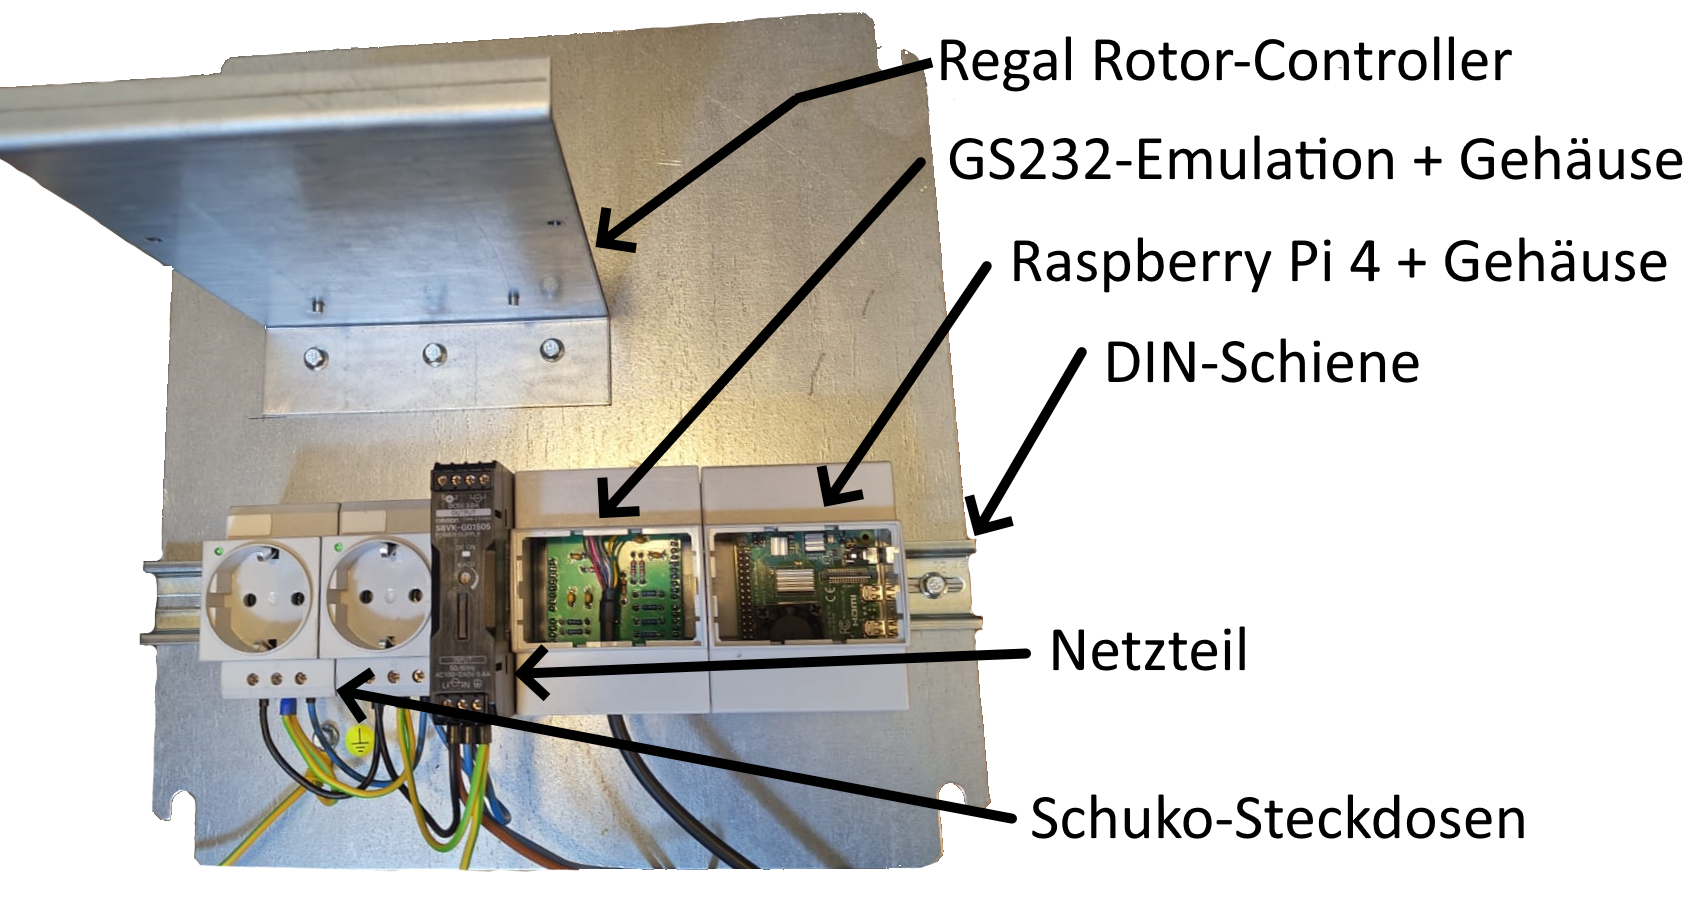
\includegraphics[width=0.7\linewidth]{../ref/Schaltschrank_Befestigung.jpg}
	\caption{Befestigungskonzept im Schaltschrank}
	\label{fig:schaltschrankbefestigung}
\end{figure}

\subsection{Anschlüsse am Schaltschrank}
Der Schaltschrank verfügt an der Außenseite über keinerlei Anschlüsse. Die Kabel für die Stromversorgung, Antenne und Rotoren verlaufen über Kabelverschraubungen nach außen, um dort direkt verwendet werden zu können. 

\begin{figure}[H]
	\centering
	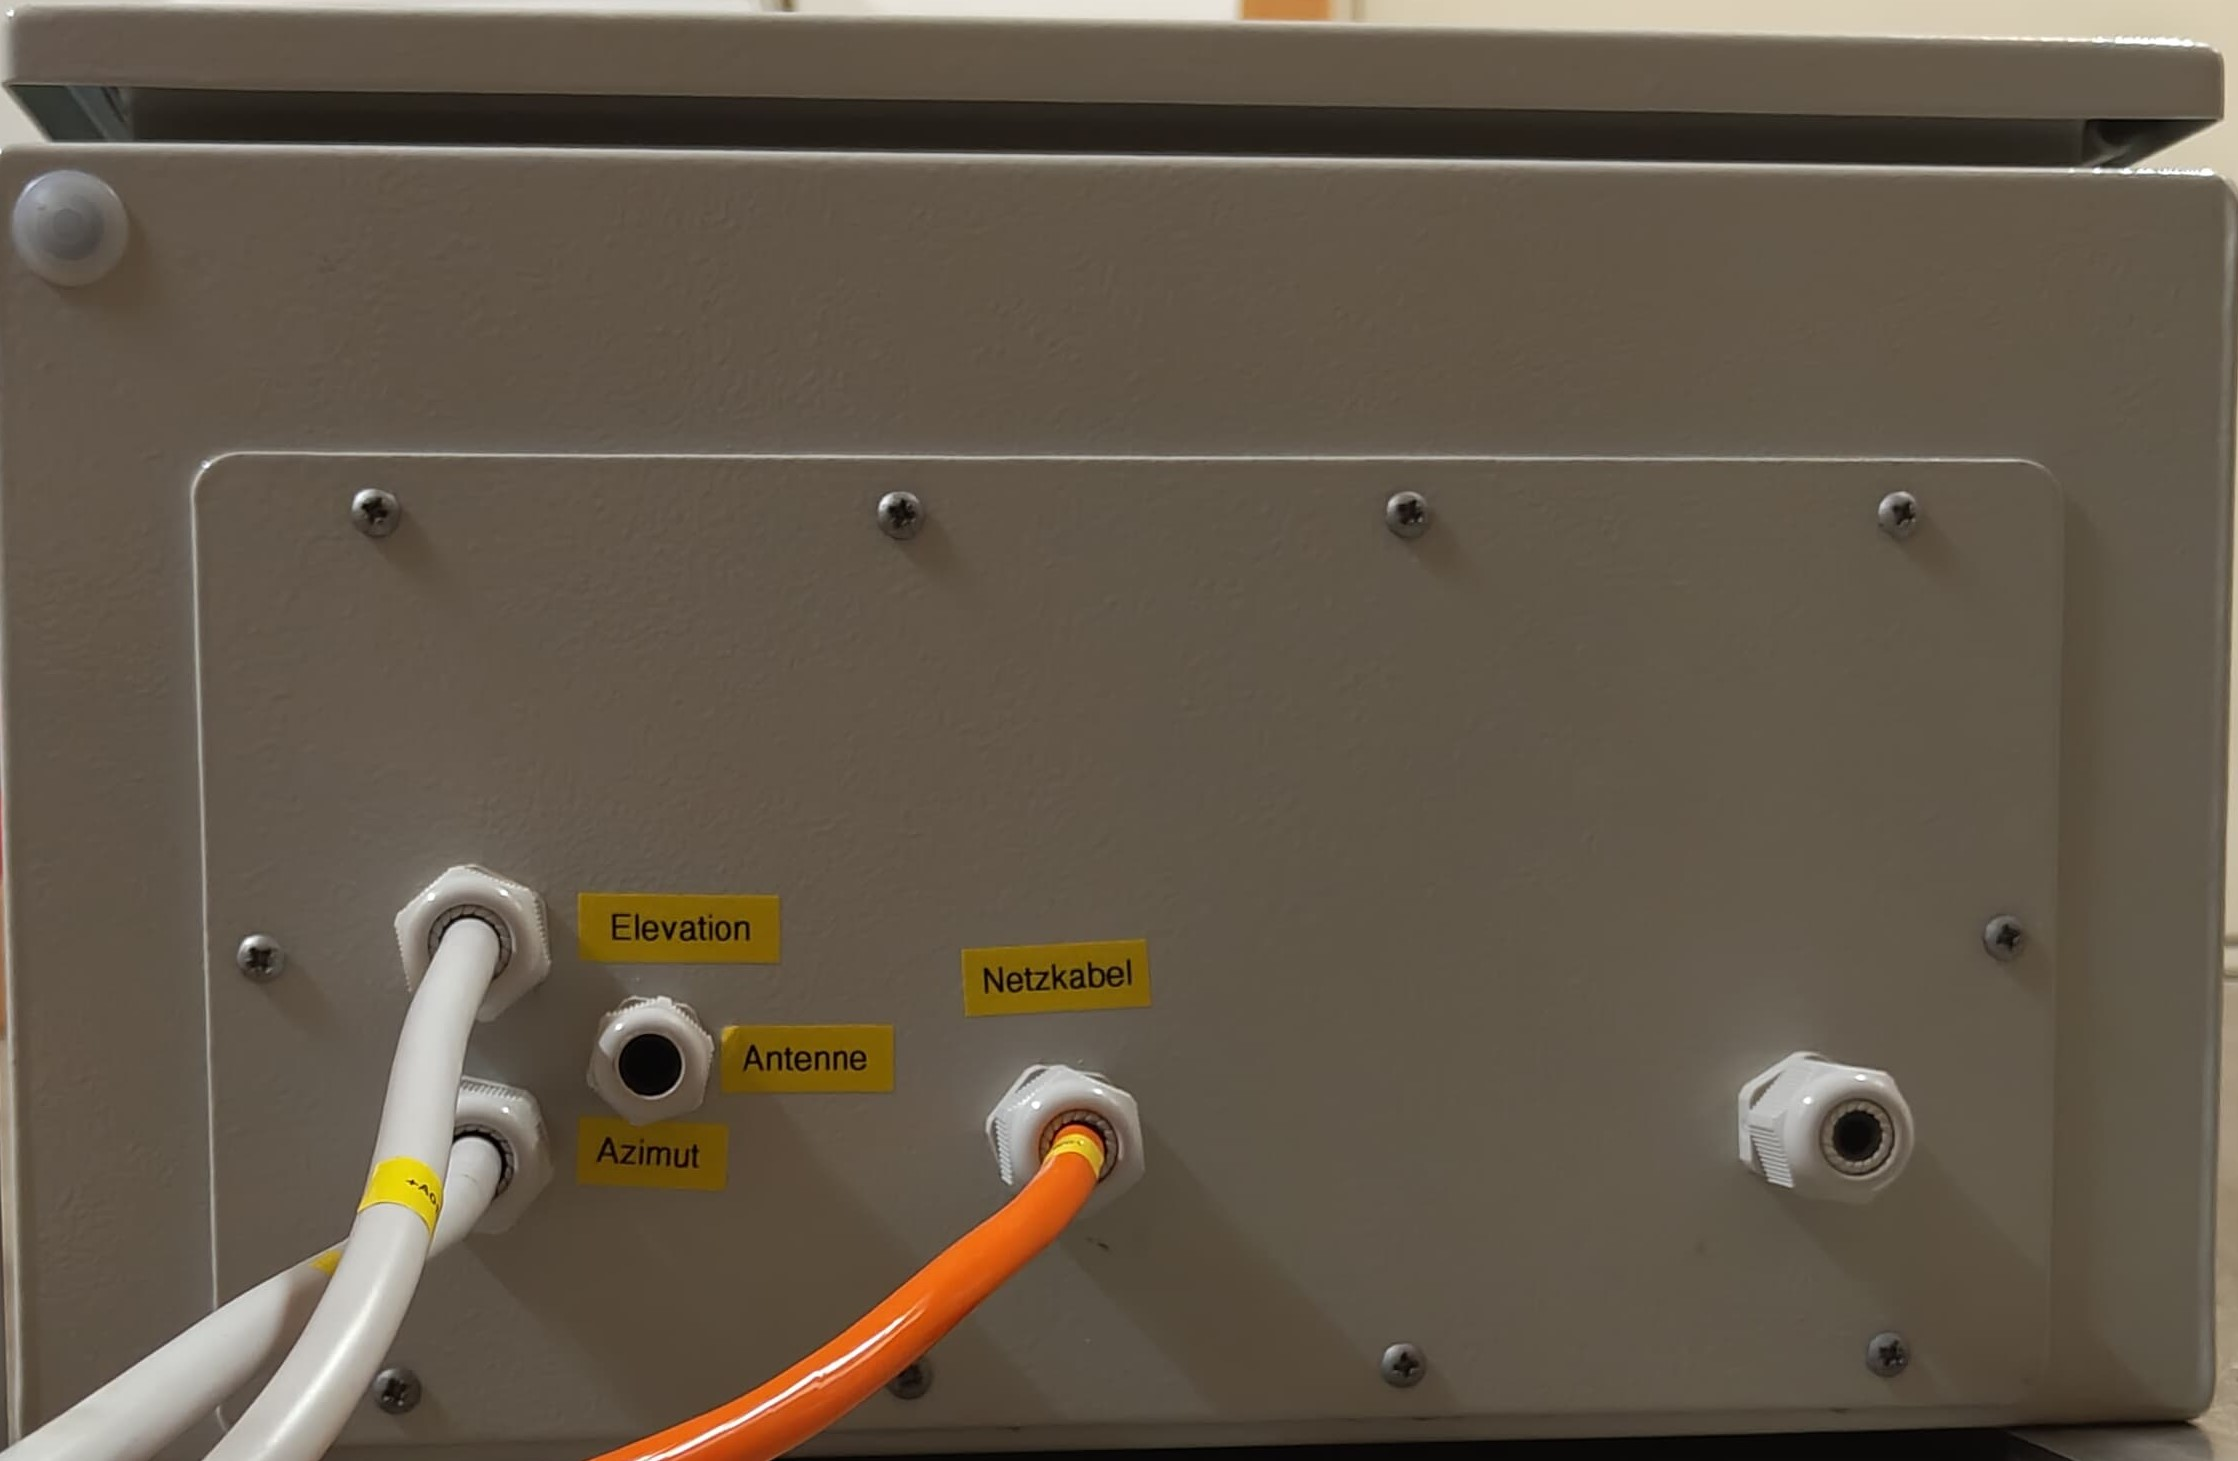
\includegraphics[width=0.7\linewidth]{../ref/Schaltschrank_Anschluss.jpeg}
	\caption{Anschlüsse am Schaltschrank}
	\label{fig:schaltschrankanschluesse}
\end{figure}

Die unbeschriftete Schraubverbindung in Abbildung \ref{fig:schaltschrankanschluesse} dient als Reserve für mögliche Erweiterungen.

\subsection{Standfüße}
Um den Schaltschrank flexibel platzieren zu können, werden zwei Standfüße aus 10 Millimeter Chromstahlblech zusammengeschweißt und mit Gummifüßen versehen. 

\begin{figure}[H]
	\centering
	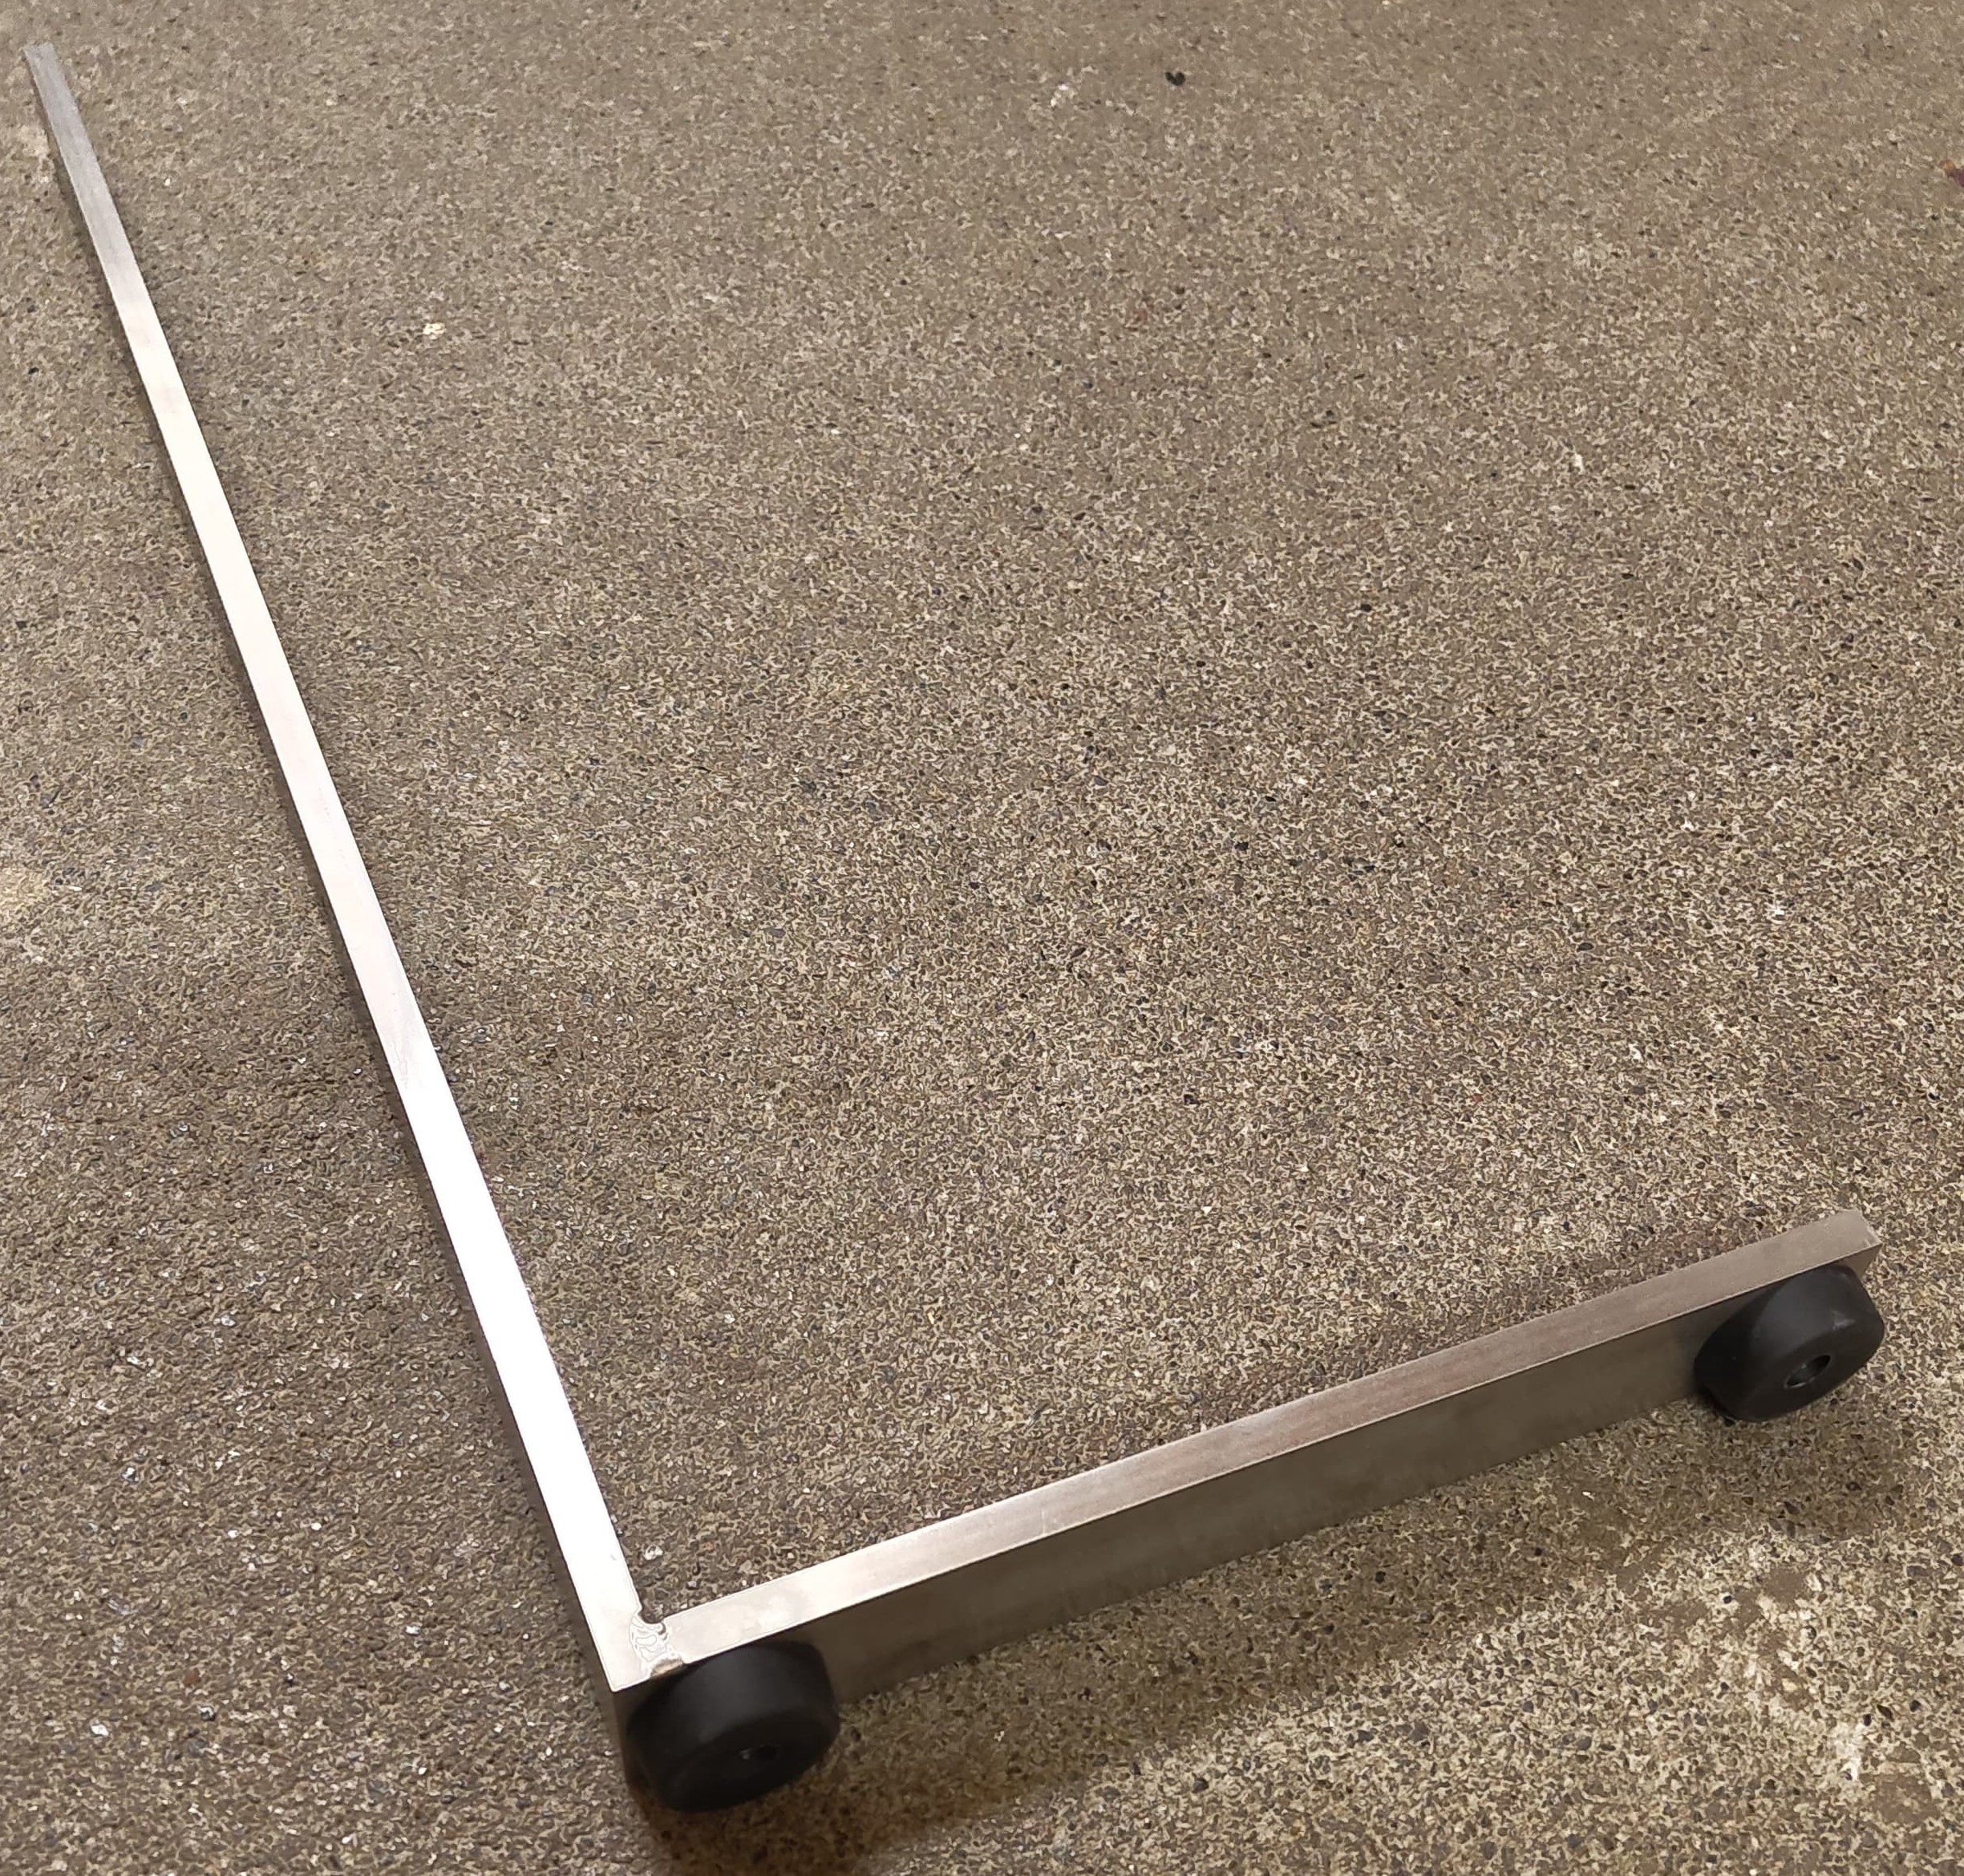
\includegraphics[width=9cm]{../ref/Schaltschrank_Fuss.jpeg}
	\caption{Standfuß für den Schaltschrank}
	\label{fig:schaltschrankfuss}
\end{figure}

Das Ergebnis ist ein modular platzierbarer und vielseitiger Schaltschrank:

\begin{figure}[H]
	\begin{minipage}[b]{.4\linewidth}
		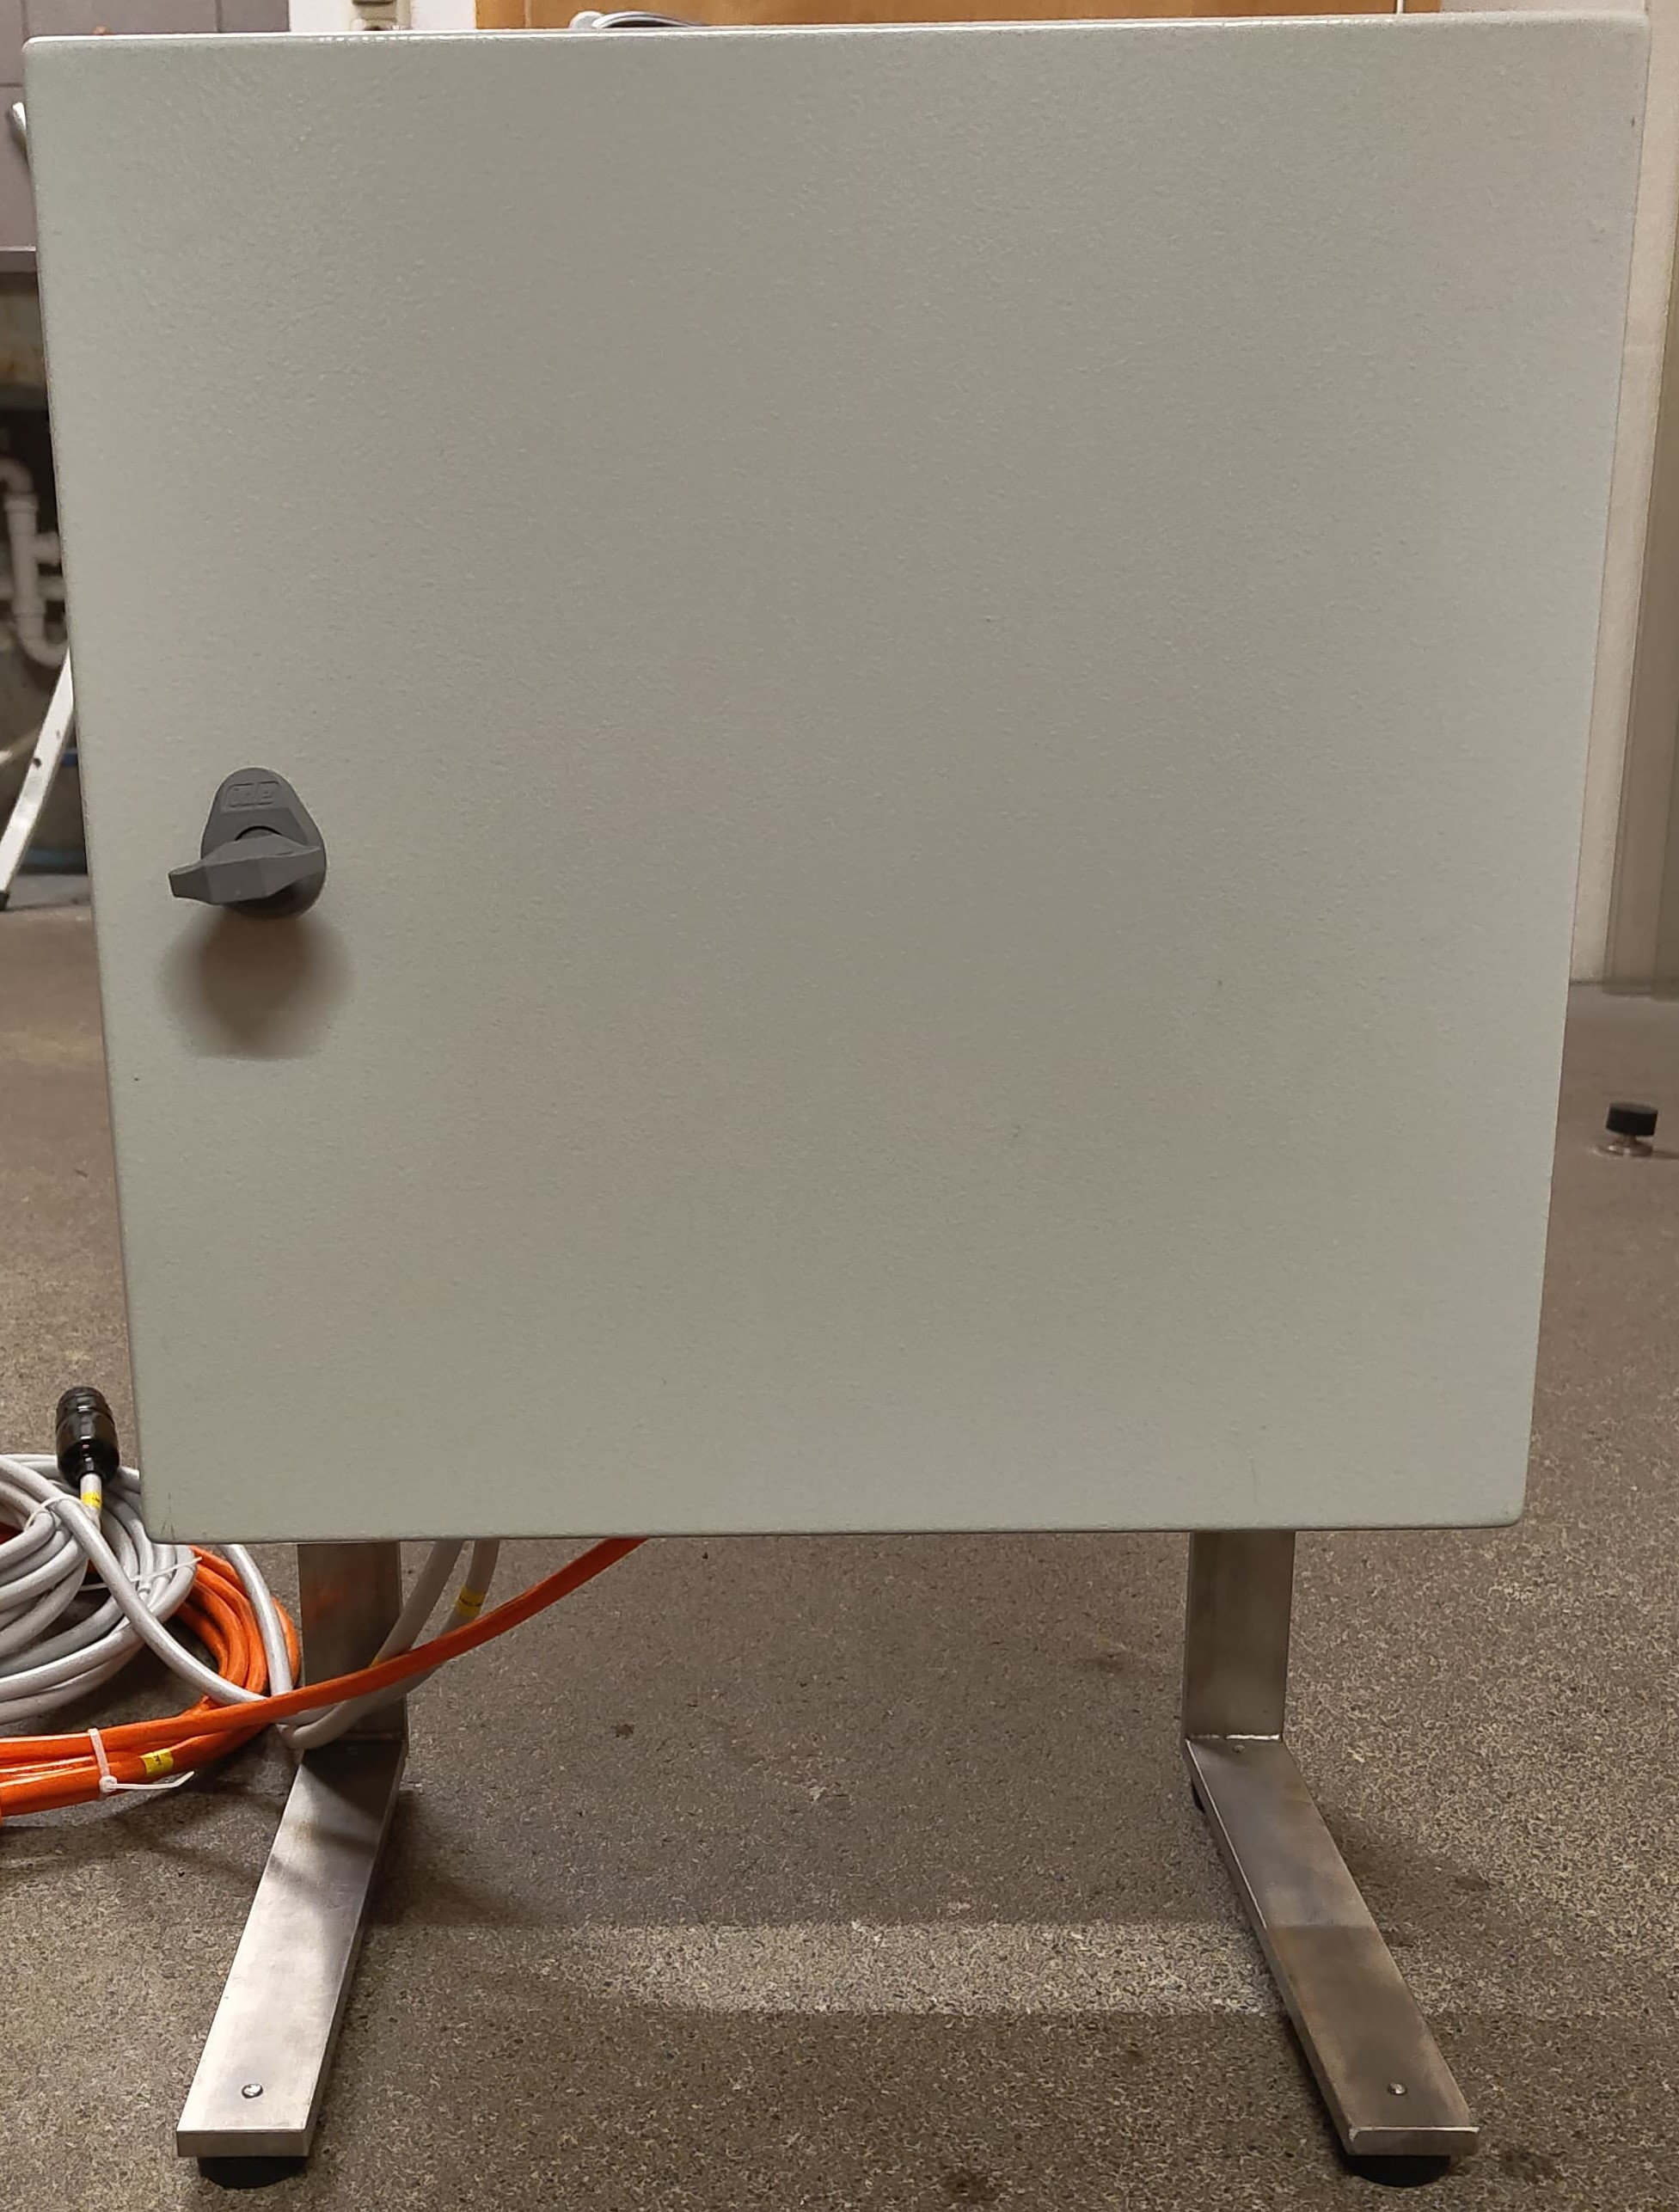
\includegraphics[width=\linewidth]{../ref/Schaltschrank_stehend_vorne.jpeg}
		\label{fig:schaltschrankstehendvorne}
		\caption{Schaltschrank stehend (Ansicht vorne)}
	\end{minipage}
	\hspace{.1\linewidth}% Abstand zwischen Bilder
	\begin{minipage}[b]{.4\linewidth} % [b] => Ausrichtung an \caption
		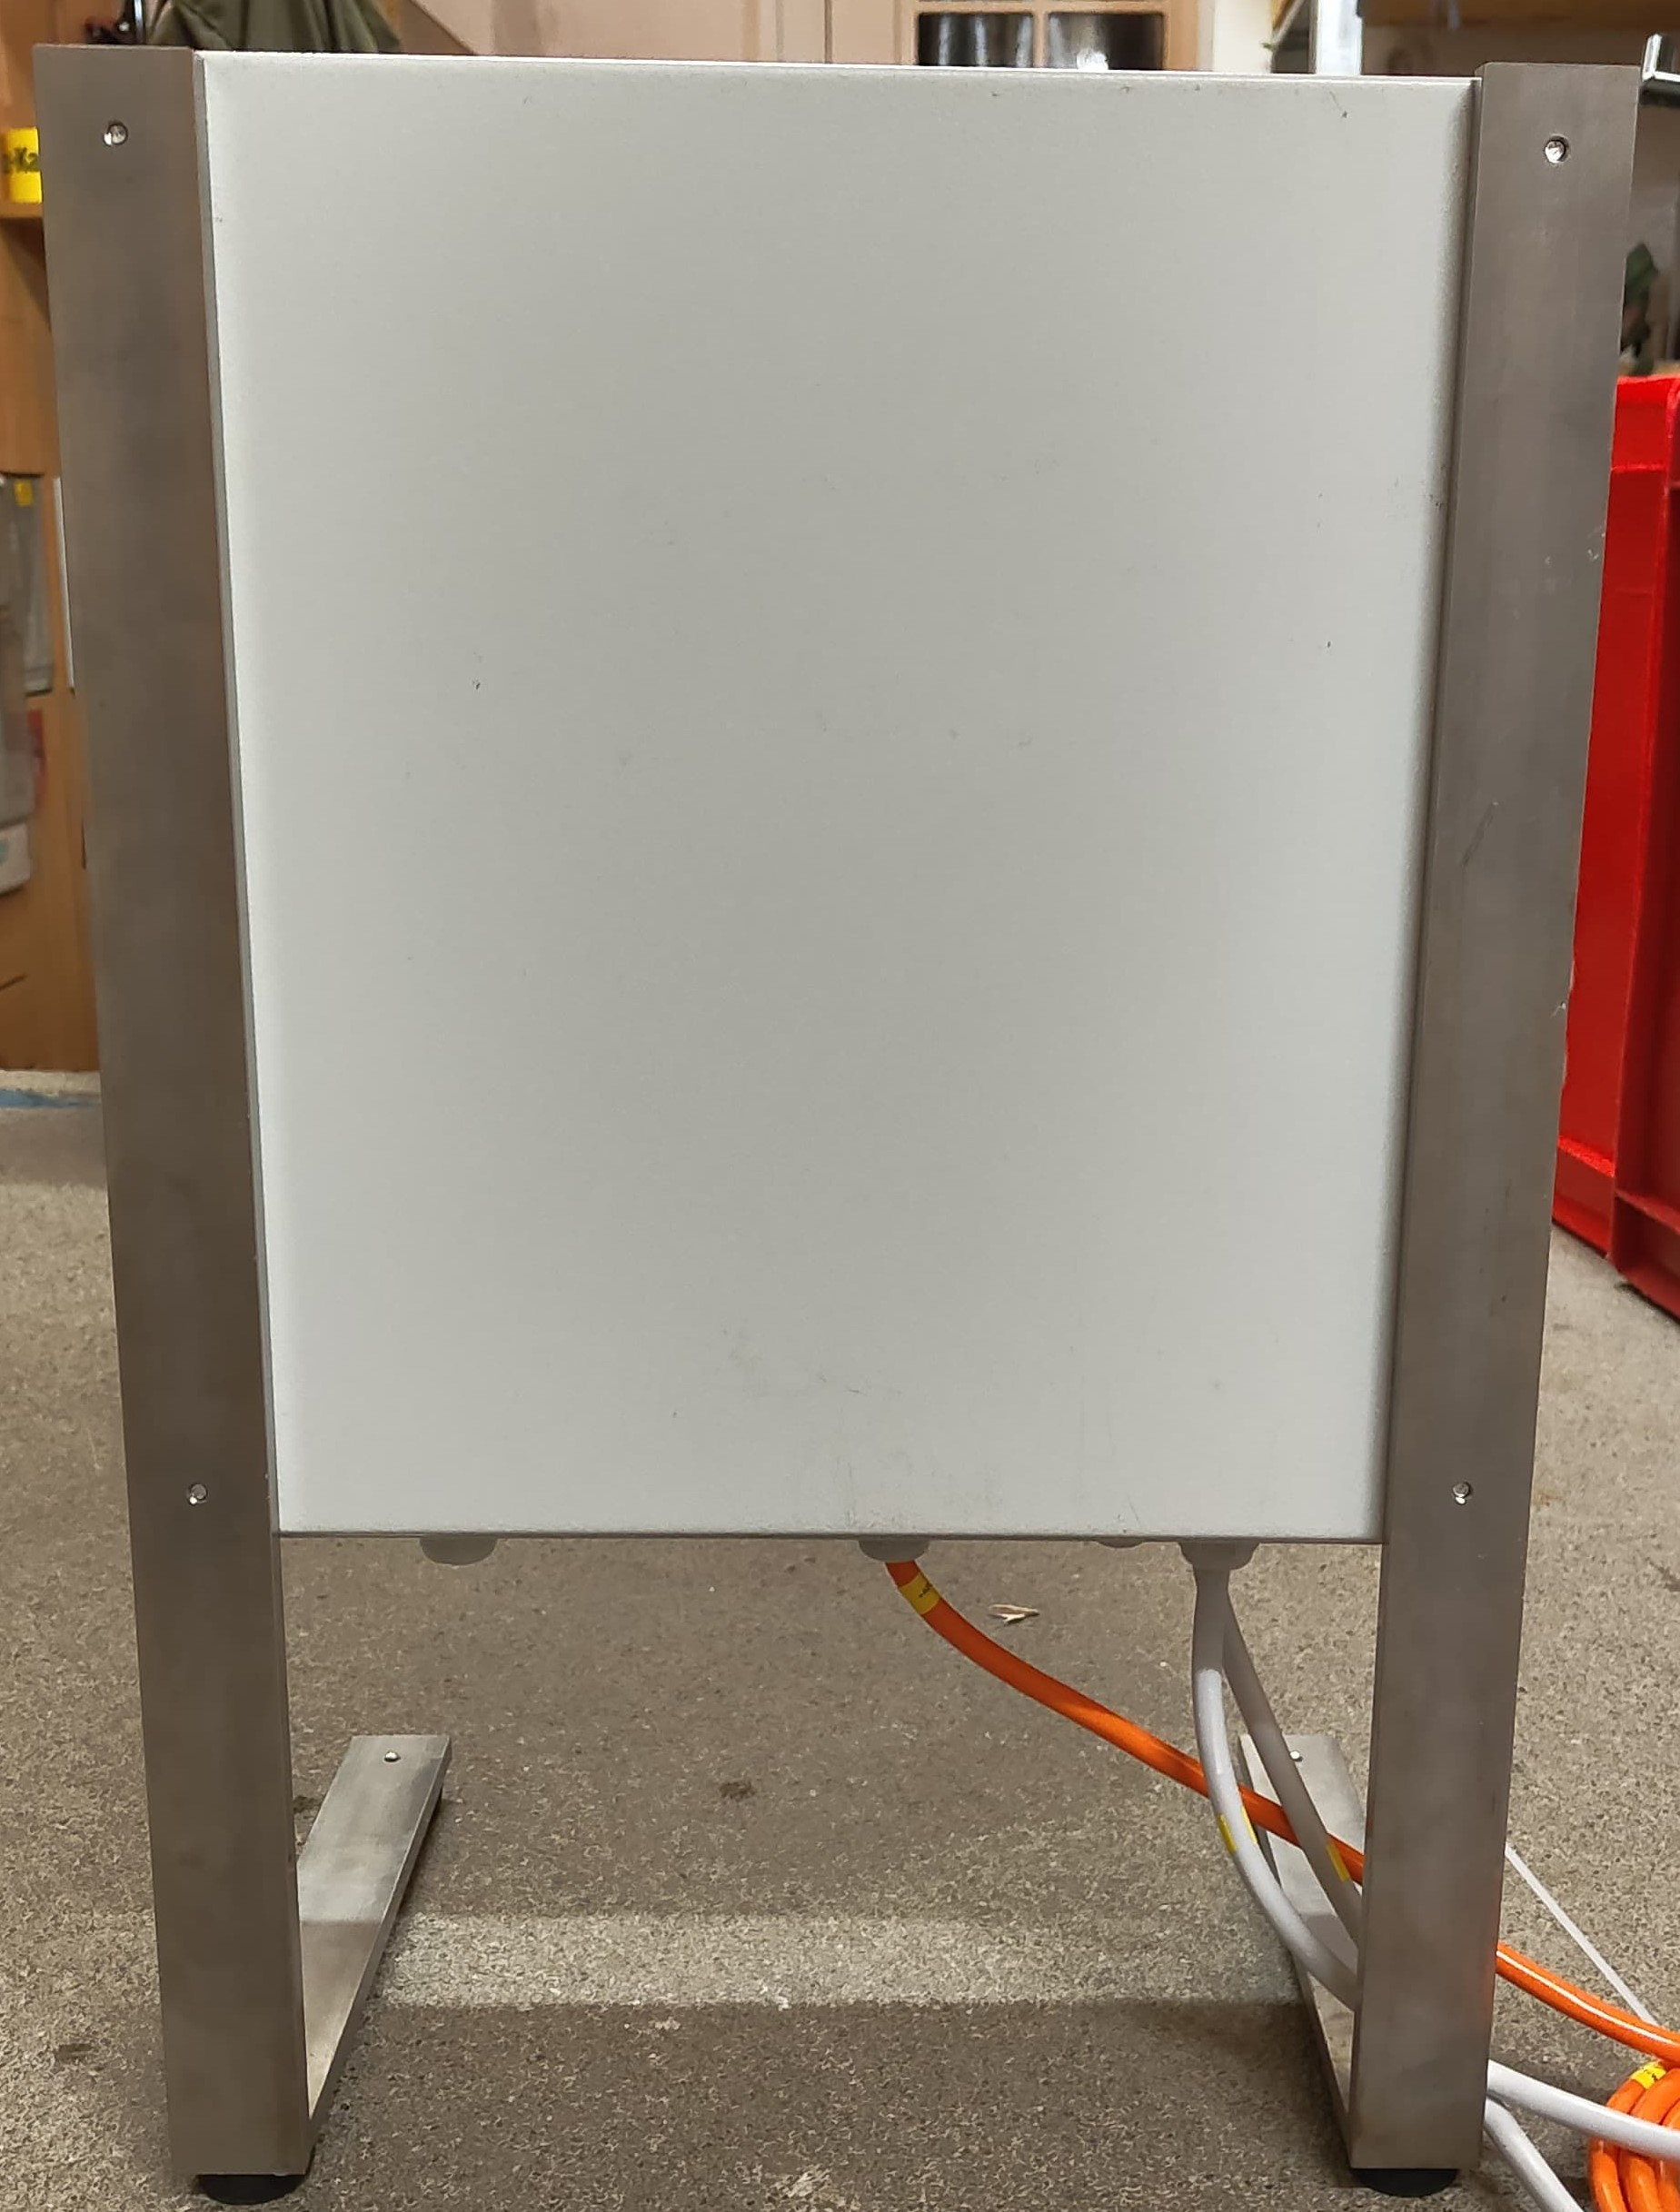
\includegraphics[width=\linewidth]{../ref/Schaltschrank_stehend_hinten.jpeg}
		\label{fig:schaltschrankstehendhinten}
		\caption{Schaltschrank stehend (Ansicht hinten)}
	\end{minipage}
\end{figure}

\begin{figure}[H]
	\centering
	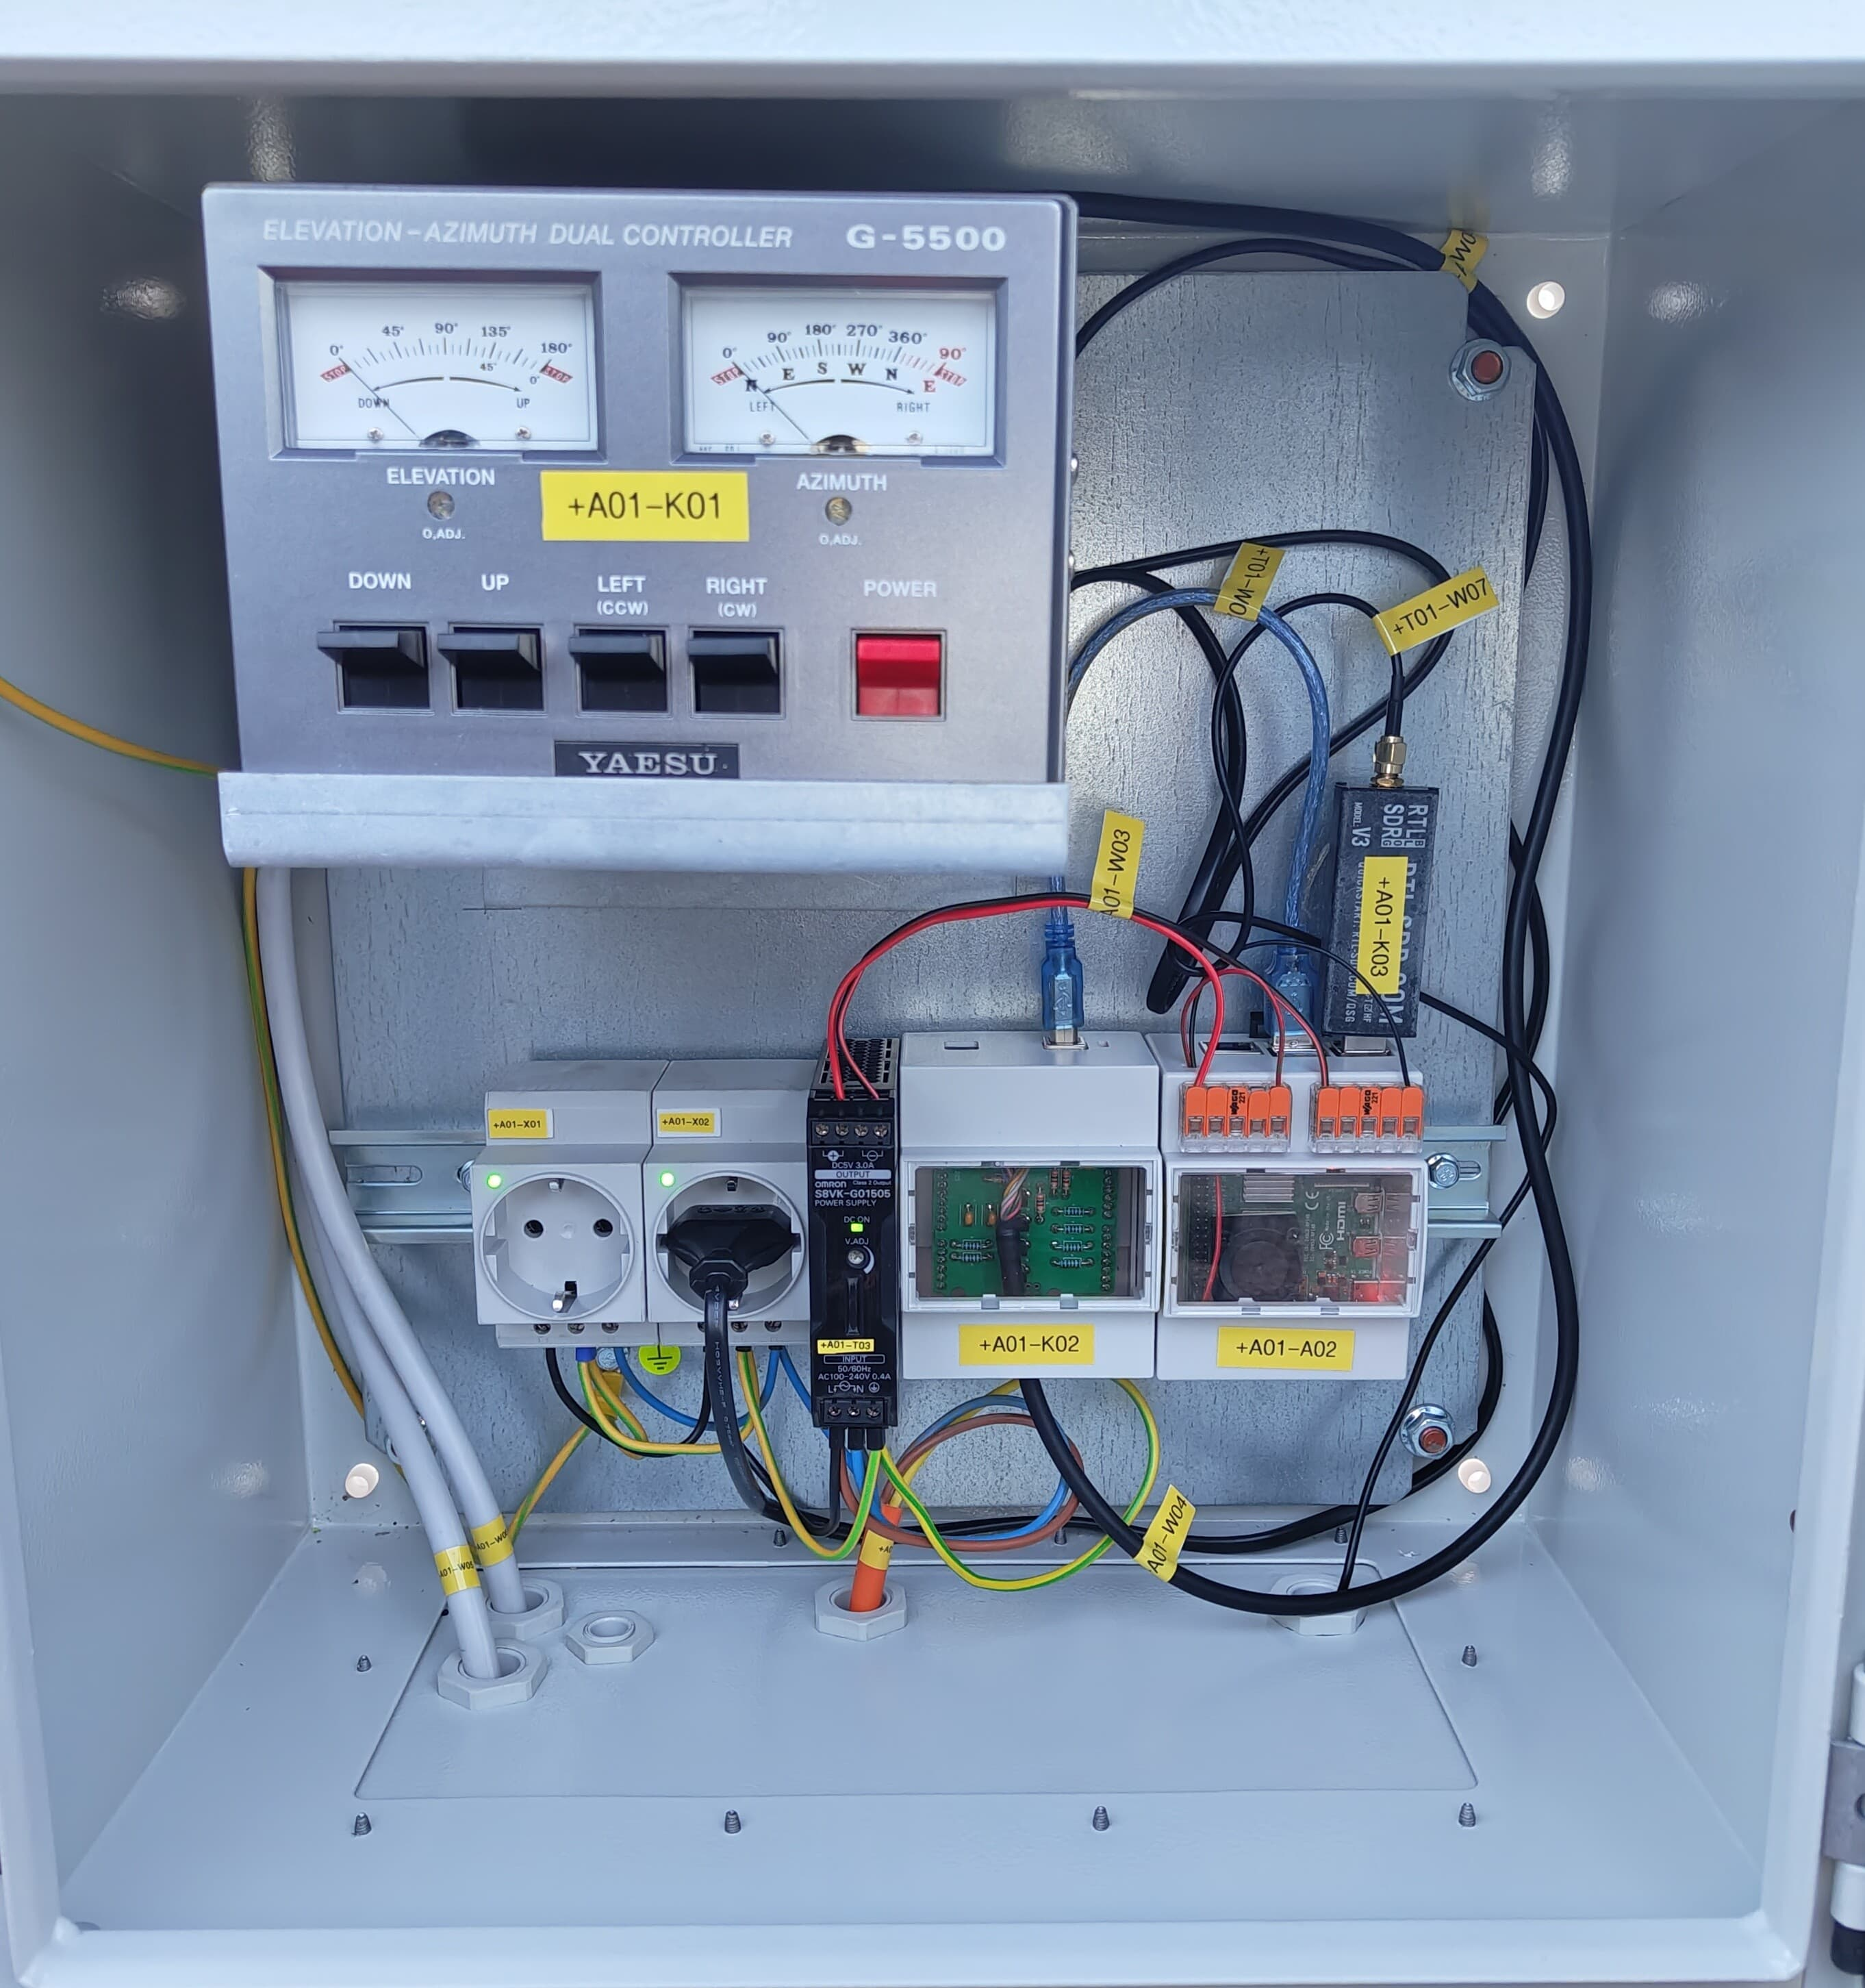
\includegraphics[width=.5\linewidth]{../ref/schaltschrank_innen.jpeg}
	\caption{Innenansicht des fertig verkabelten Schaltschranks}
	\label{fig:schaltschrankinnen}
\end{figure}

\section{SDR}
\label{sec:sdr}
SDRs ersetzen traditionelle Hardwarekomponenten für Hochfrequenzsender und -empfänger durch Software, um Signale zu empfangen, zu demodulieren und zu verarbeiten. Anstatt spezielle Hardware für jede Funkkommunikationsart zu benötigen, kann ein SDR flexibel über eine Software konfiguriert werden und somit verschiedene Frequenzen und Modulationsarten unterstützen. Durch die Digitalisierung des Funkempfangs ermöglicht ein SDR eine breite Palette von Anwendungen und verbesserte Flexibilität bei der Signalverarbeitung. \cite{noauthor_sdr_nodate}

Das für diese Empfangsstation verwendete SDR ist das RTL-SDR Blog v3 mit folgenden Spezifikationen:
\begin{table}[H]
	\centering
	\begin{tabular}{ll}
		\textbf{Bandbreite} & bis zu 2.4 Megahertz \\
		\textbf{ADC} & RTL2832U 8-Bit \\
		\textbf{Frequenzbereich} & 500 Kilohertz bis 1766 Megahertz \\
		\textbf{typischer Eingangswiderstand} & 50 Ohm \\
		\textbf{typische Stromaufnahme} & 270 bis 280 Milliampere \\
		\textbf{steuerbares Bias-T} & Ja (4.5 Volt) \\
	\end{tabular}
\end{table}

Das RTL-SDR Blog v3 wird über einen USB-B Stecker zum Raspberry Pi 4 verbunden und verfügt über einen SMA-Stecker für den Anschluss der Antenne. \cite{noauthor_rtl-sdr_nodate}

\section{Netzteil}
\label{sec:Netzteil}
Für die Stromversorgung des Raspberry Pi 4 sowie des im GS232A/B verbauten Arduino Uno wird das Schaltnetzteil S8VK-G01505 der OMRON Corporation verwendet. Das Netzteil kann mit einer Eingangsspannung von 100 bis 240 Volt und 50 Hertz betrieben werden und sorgt für eine Ausgangsspannung von 5 Volt. Mit einer maximalen Ausgangsleistung von 15 Watt ist es ausreichend groß dimensioniert, um sowohl den Raspberry Pi 4 \cite{noauthor_power_nodate} als auch den Arduino Uno \cite{noauthor_r3_nodate} mit Strom zu versorgen. \cite{noauthor_s8vk-g01505_nodate}

\section{Netzkabel}
\label{sec:Netzkabel}
Das Netzkabel, mit einer Länge von 4.6 Metern außerhalb des Schaltschranks, versorgt die gesamte Empfangsstation mit Energie. Voraussetzung zum Betrieb der Empfangsstation ist es demnach, das Netzkabel mit einer Spannungsquelle (100 Volt bis 120 Volt und 50 Hz oder 200 Volt bis 240 Volt und 50 Hz) zu verbinden. Das verwendete Kabel ist ein H07BQ-F 3G1.5 der PATELEC Group \cite{noauthor_cables_nodate} und weist dank dem verwendeten Mantelmaterial Polyurethan eine gute UV-Beständigkeit auf \cite{noauthor_polyurethan_nodate}.

\section{USB-Kabel}
\label{sec:USB-Kabel}
Das USB-Kabel ist ein USB-A zu USB-B Kabel und verbindet den Raspberry Pi 4 (USB-A) mit dem Arduino Uno (USB-B) der GS232-Interface Emulation. Abgesehen von der Kommunikation zwischen dem Raspberry Pi 4 und dem Arduino Uno erfolgt auch die Stromversorgung des Arduinos über das USB-Kabel. Es handelt sich bei dem USB-Kabel um ein handelsübliches Kabel aus dem Eigenbestand ohne spezielle Eigenschaften, da es im Schaltschrank keinerlei mechanischen Belastung ausgesetzt ist.

\section{5V-Kabel}
\label{sec:5V-Kabel}
Die Aufgabe des 5V-Kabels ist die Energieübertragung vom Netzteil zum Raspberry Pi 4. Dazu wird die verwendete rot-schwarze Zwillingsleitung vom Ausgang des Netzteil zu den auf dem Gehäuse angebrachten Verbindungsklemmen geführt. Der Zwischenschritt über die Verbindungsklemmen ermöglicht nicht nur ein leichteres Ein- und Ausbauen der Komponenten, sondern fördert auch die Skalierbarkeit im Bezug auf den Einbau weiterer elektronischer Komponenten, welche eine 5 Volt Versorgungsspannung benötigen.

\begin{figure}[H]
	\centering
	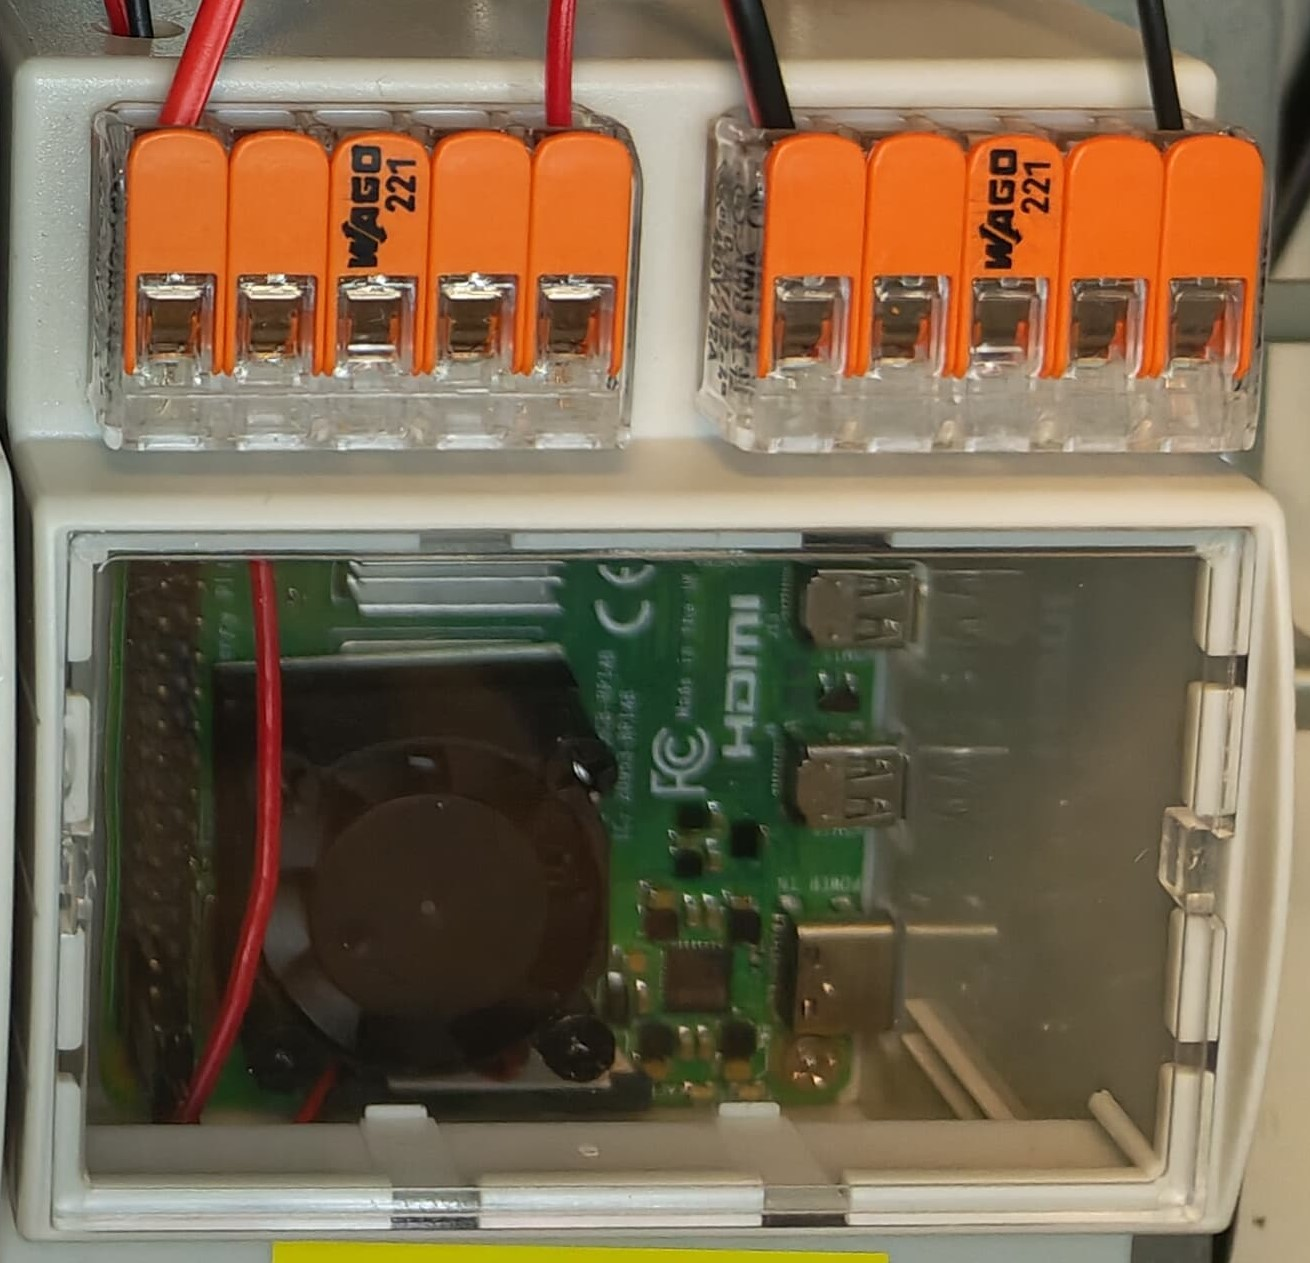
\includegraphics[width=.25\linewidth]{../ref/Anschlussklemmen5V.jpeg}
	\caption{Anschlussklemmen 5 Volt Versorgung}
	\label{fig:anschlussklemmen}
\end{figure}

\section{DIN-Kabel}
\label{sec:DIN-Kabel}
Als DIN-Kabel wird in diesem Fall jenes Kabel bezeichnet, welches zur Verbindung der GS232-Interface Emulation zum G-5500DC Controller verwendet wird und an einem Ende einen 8-Pol DIN-Rundstecker aufweist. Die Zuordnung der Farben des Kabels zu den PIN-Nummern des Steckers, die im Kapitel \ref{subsubsec:emulation_analoge_schnittstelle} genauer erläutert wurde, sowie die Zuordnung zu den Bezeichnungen auf dem Arduino-Shield, beschrieben im Kapitel \ref{subsec:hardware}, lautet wie folgt:

\begin{table}
	\centering
	\begin{tabular}{c|c|c}
		\textbf{Farbe} & \textbf{Pin-Nummer} & \textbf{Bezeichnung am Arduino-Shield} \\
		\hline
		Grün & 1 & V \\
		Gelb & 2 & R \\
		Grau & 3 & U \\
		Weiß & 4 & L \\
		Blau & 5 & D \\
		Pink & 6 & H \\
		Rot & 7 & Vin \\
		Braun & 8 & GND \\
	\end{tabular}
\end{table}

\section{Azimut-Kabel}
\label{sec:azimutkabel}
Das Azimut-Kabel dient zur Steuerung und Messung der Ausrichtung des Azimut-Rotors. Als Kontrollkabel bezeichnet wird seine Funktion im Kapitel \ref{subsubsec:kontrollkabel} beschrieben. Mit einem Leiterquerschnitt von je 1.5 Millimetern erfüllt es die in Kapitel \ref{subsubsec:kontrollkabel} genannten Vorgaben und ist aufgrund des UV-stabilisierten Außenmantels aus Polyvinylchlorid auch gegen irreparable Schäden durch Sonneneinstrahlung geschützt. Die Länge des Kabels außerhalb des Schaltschranks beträgt 4.8 Meter. 

\section{Elevation-Kabel}
\label{sec:Elevation-Kabel}
Das Elevation-Kabel ist das Pendant zum Azimut-Kabel und dient der Steuerung und Messung der Ausrichtung des Elevation-Rotors. Die Eigenschaften entsprechen dem im Kapitel \ref{sec:azimutkabel} beschriebenen Eigenschaften des Azimut-Kabel.

\section{Schuko 1}
\label{sec:schuko1}
Die Schutzkontaktsteckdose dient der Energieversorgung von Geräten mit Netzstecker. Das verwendete Modell SD35DEA des Unternehmen SHC GmbH verfügt über eine grüne Status-LED, die leuchtet, sobald das Netzkabel des Schaltschranks an eine Energiequelle angeschlossen wird. Die Schutzkontaktsteckdose Schuko 1 ist als Reserve für mögliche weitere Geräte oder für temporäre Anwendungen wie zum Beispiel das Laden eines Notebooks oder dem Ausleuchten des Schaltschranks eingebaut.

\section{Schuko 2}
\label{sec:schuko2}
Die Schutzkontaktsteckdose Schuko 2 weist dieselben technischen Eigenschaften wie die Schutzkontaktsteckdose Schuko 1, welche in Kapitel \ref{sec:schuko1} beschrieben wird, auf und ist für die Energieversorgung des Yeasu G-5500DC Controllers vorgesehen, kann allerdings auch für jegliche andere Geräte verwendet werden.

\section{Antennenkabel Helix und Array}
\label{sec:Antennenkabel-Helix}
Die Antennenkabel +A03-W09 bis W12 des Typ RG58 C/U führen von den Antennen zum RF-Combiner mit einer Länge von insgesamt 1.25 Meter pro Kabel. Entsprechend der RG58 C/U Bezeichnung weisen die Kabel einen Wellenwiderstand von 50 Ohm \cite{noauthor_rg_nodate} sowie eine Dämpfung von 0.3 Dezibel pro Meter bei 400 Megahertz auf. \cite{noauthor_vergleich_nodate}. 

\section{LNA}
\label{sec:LNA}
Die Leistung einer Antenne lässt sich in einer Gütezahl angeben, die als gain-to-noise-temperature, kurz G/T, bezeichnet wird. G/T ist eine positive Zahl, welche mit steigender Performanz der Antenne zunimmt. Um diese Gütezahl zu verbessern, muss entweder der Gewinn der Antenne vergrößert oder der relative Rauschanteil im Signal verringert werden. Weil sich das Vergrößern des Gewinns einer omnidirektionalen Antenne als sehr schwierig gestaltet und in den meisten Fällen in einer gerichteten Antenne mündet, muss der Rauschanteil abnehmen. Um dies zu erreichen wird das Wideband LNA von RTL-SDR.com in der Signalkette direkt nach der Antenne verwendet. Im Vergleich zum SDR, welches ursprünglich als einzige Komponente die Aufgabe hatte das Signal der Antenne zu Verstärken, weist das Wideband LNA mit 0.52 Dezibel bei 800 MHz eine sehr geringe Rauschzahl auf. \cite{noauthor_new_nodate} \cite{noauthor_omnidirectional_nodate}

\begin{figure}[H]
	\centering
	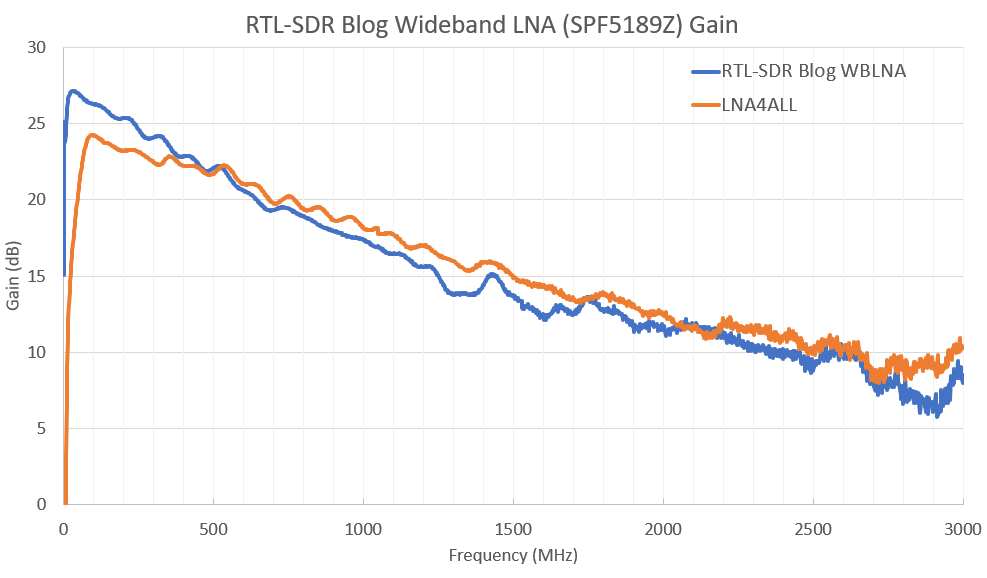
\includegraphics[width=.75\linewidth]{../ref/wideband_lna_gain.png}
	\caption{Verstärkung des Wideband LNAs in Abhängigkeit der Frequenz \cite{noauthor_new_nodate}}
	\label{fig:wideband_lna_gain}
\end{figure}

Die Verstärkung des Wideband LNAs entspricht laut Abbildung \ref{fig:wideband_lna_gain} des Herstellers etwa 22.5 Dezibel bei 433 Megahertz.

Um das LNA vor den Belastungen der Natur zu schützen, wird dieses in ein kompaktes wasserdichtes Aluminiumgehäuse mit zwei Kabelverschraubungen für die beiden Antennenkabel verbaut. 

\begin{figure}[H]
	\begin{minipage}[b]{.4\linewidth}
		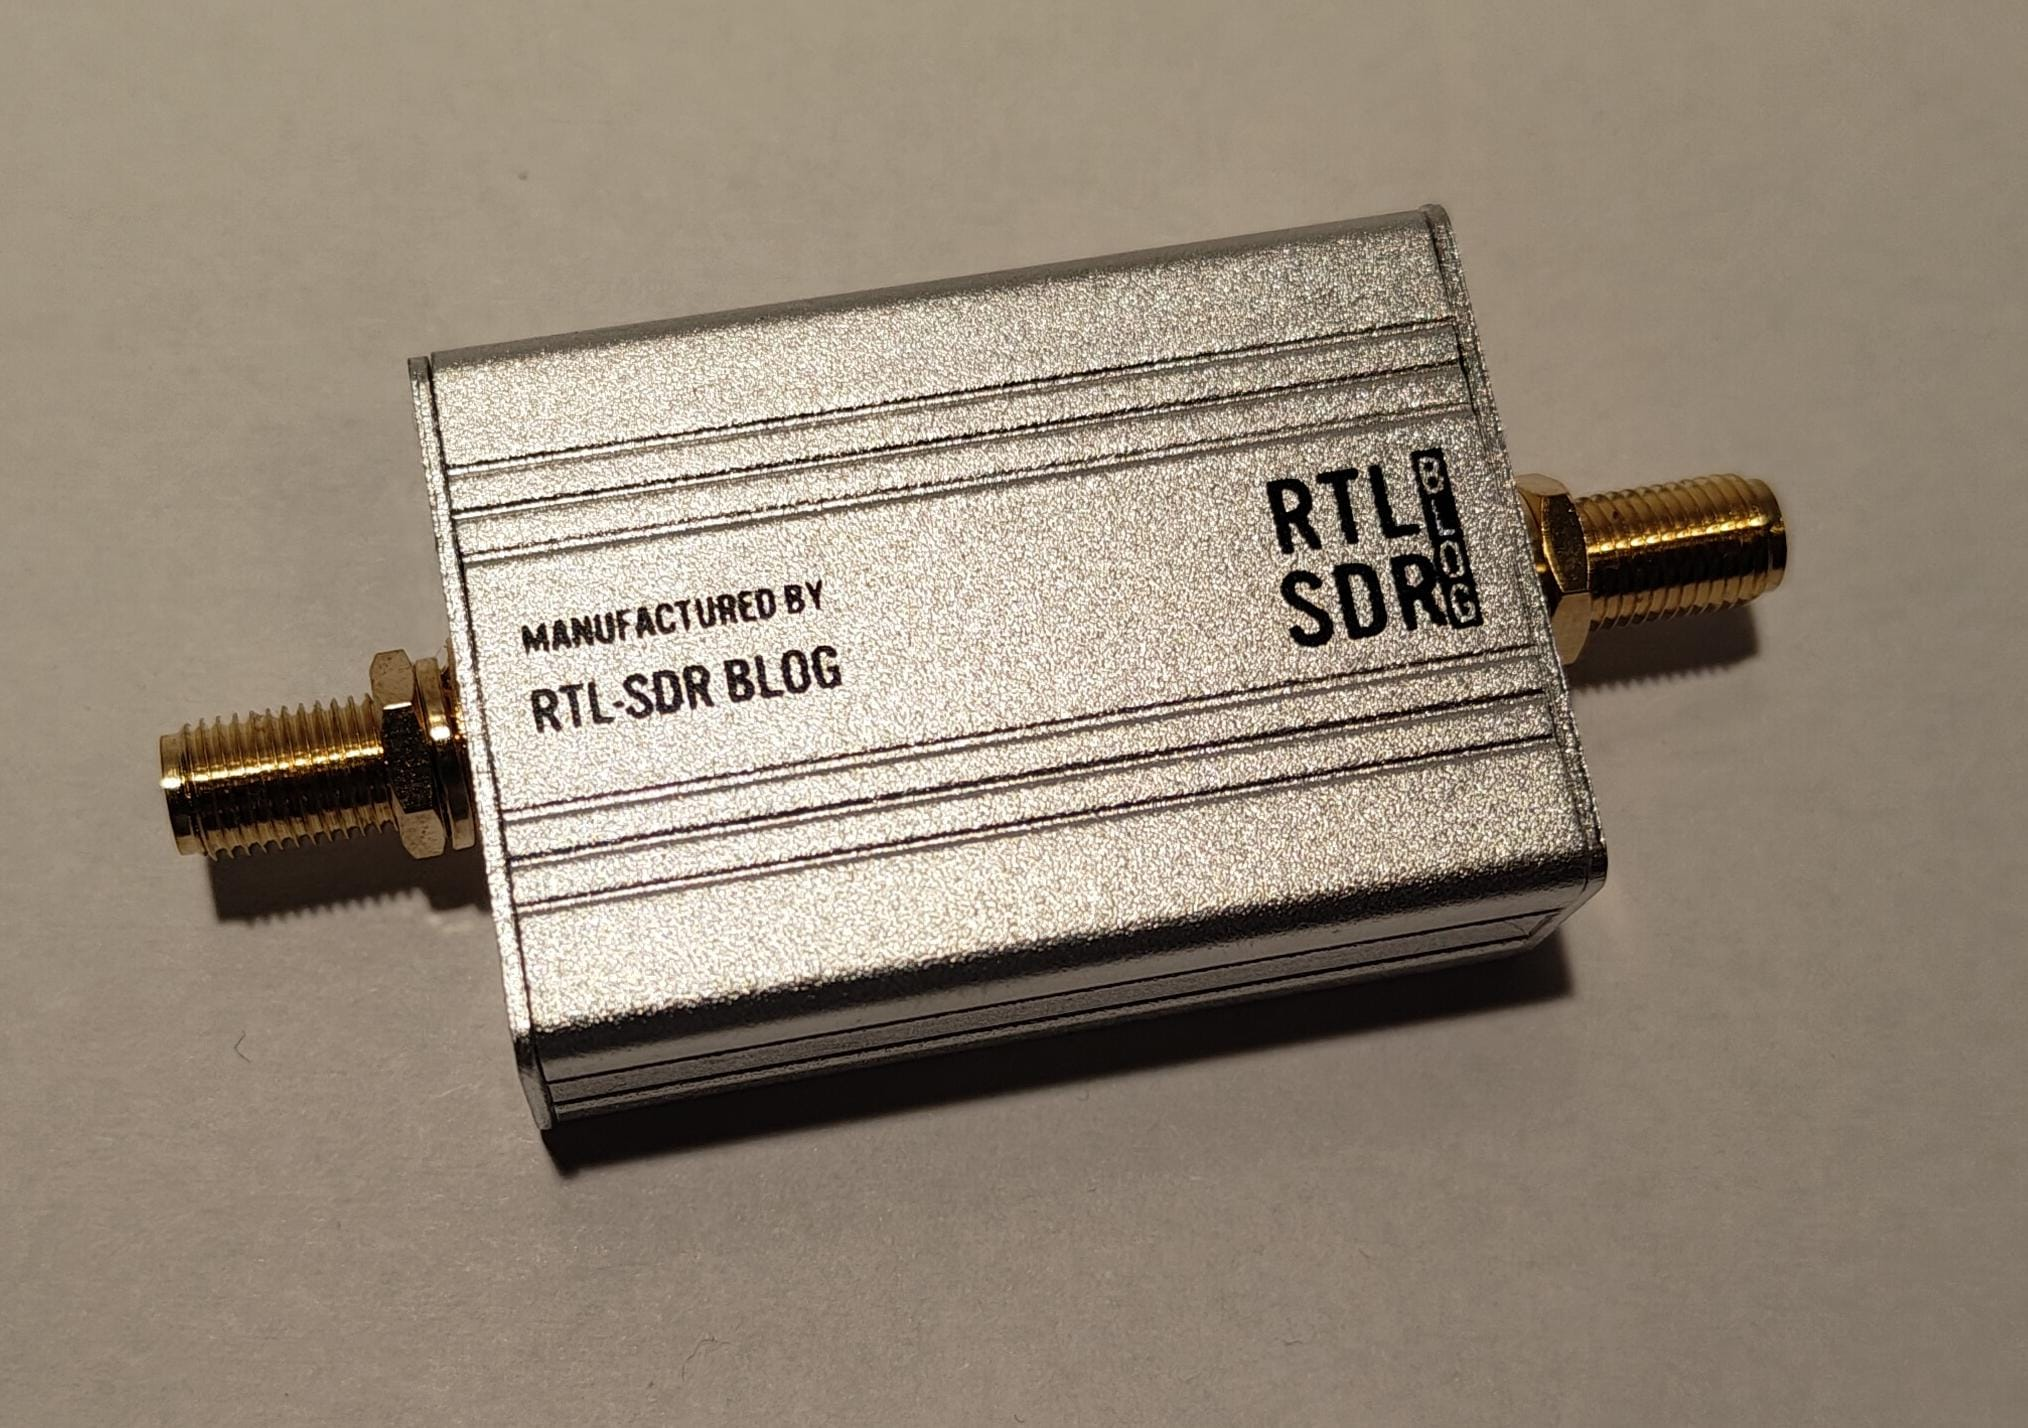
\includegraphics[width=\linewidth]{../ref/LNA.jpeg}
		\label{fig:LNA}
		\caption{Wideband LNA}
	\end{minipage}
	\hspace{.1\linewidth}% Abstand zwischen Bilder
	\begin{minipage}[b]{.4\linewidth} % [b] => Ausrichtung an \caption
		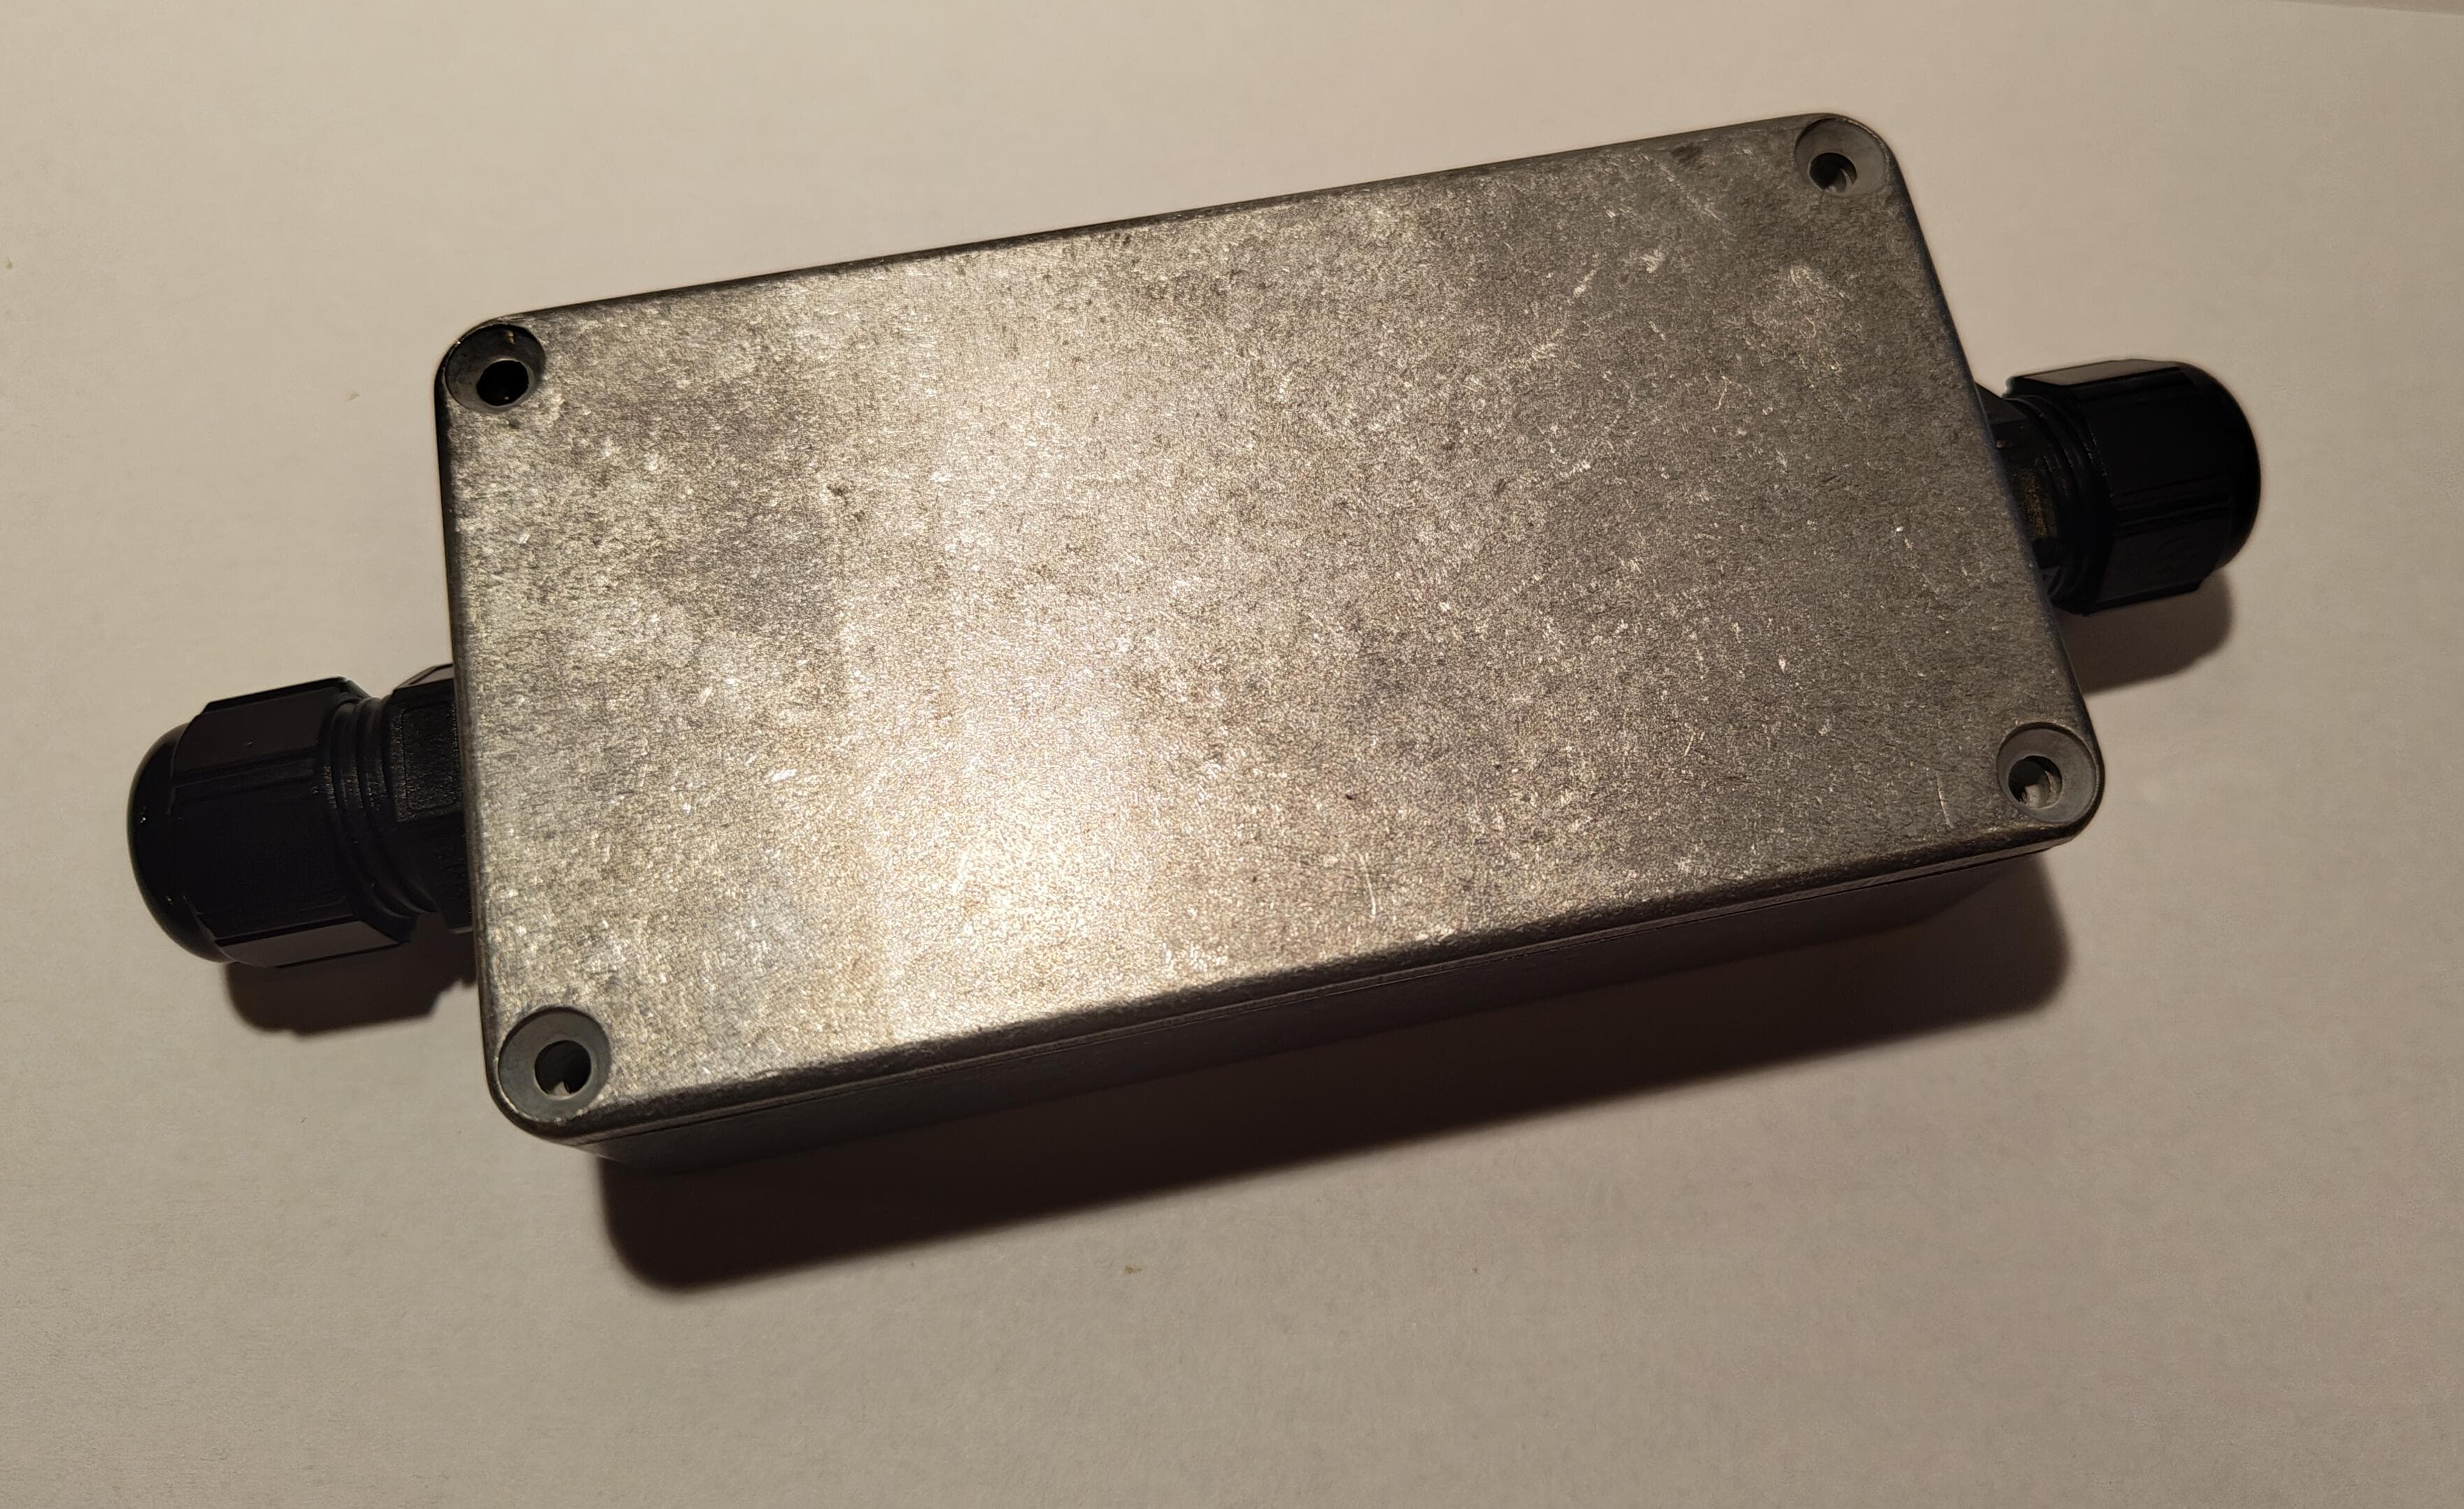
\includegraphics[width=\linewidth]{../ref/LNA_Box.jpeg}
		\label{fig:lnabox}
		\caption{Aluminiumgehäuse für das LNA}
	\end{minipage}
\end{figure}

\section{Antennen-Kabel}
\label{sec:Antennen-Kabel-QFH}
Das Antennen-Kabel +T01-W07, mit einer Länge von 3 Metern, wird für die Verbindung des SDRs mit dem Ausgang des LNAs verwendet. Das Kabel entspricht dem Typ RG174 und weist somit neben einem Wellenwiderstand von 50 Ohm eine Streckendämpfung von 0.7 Dezibel pro Meter bei 432 Megahertz auf \cite{noauthor_dunnes_nodate}.

\section{Prinzipschaltplan}
Der nachfolgende Prinzipschaltplan dient dem Zweck, Anwenderinnen und Anwendern einen guten Überblick über die verbaute Hardware und dessen Verkabelung zu geben. Die im Rahmen der Betriebsmittelkennzeichnung festgelegten Kennzeichnungen, siehe Kapitel \ref{sec:bmk}, wurden hierzu im Prinzipschaltplan berücksichtigt und die Komponenten dementsprechend beschriftet. 

\begin{landscape}
	\begin{figure}
		\centering
		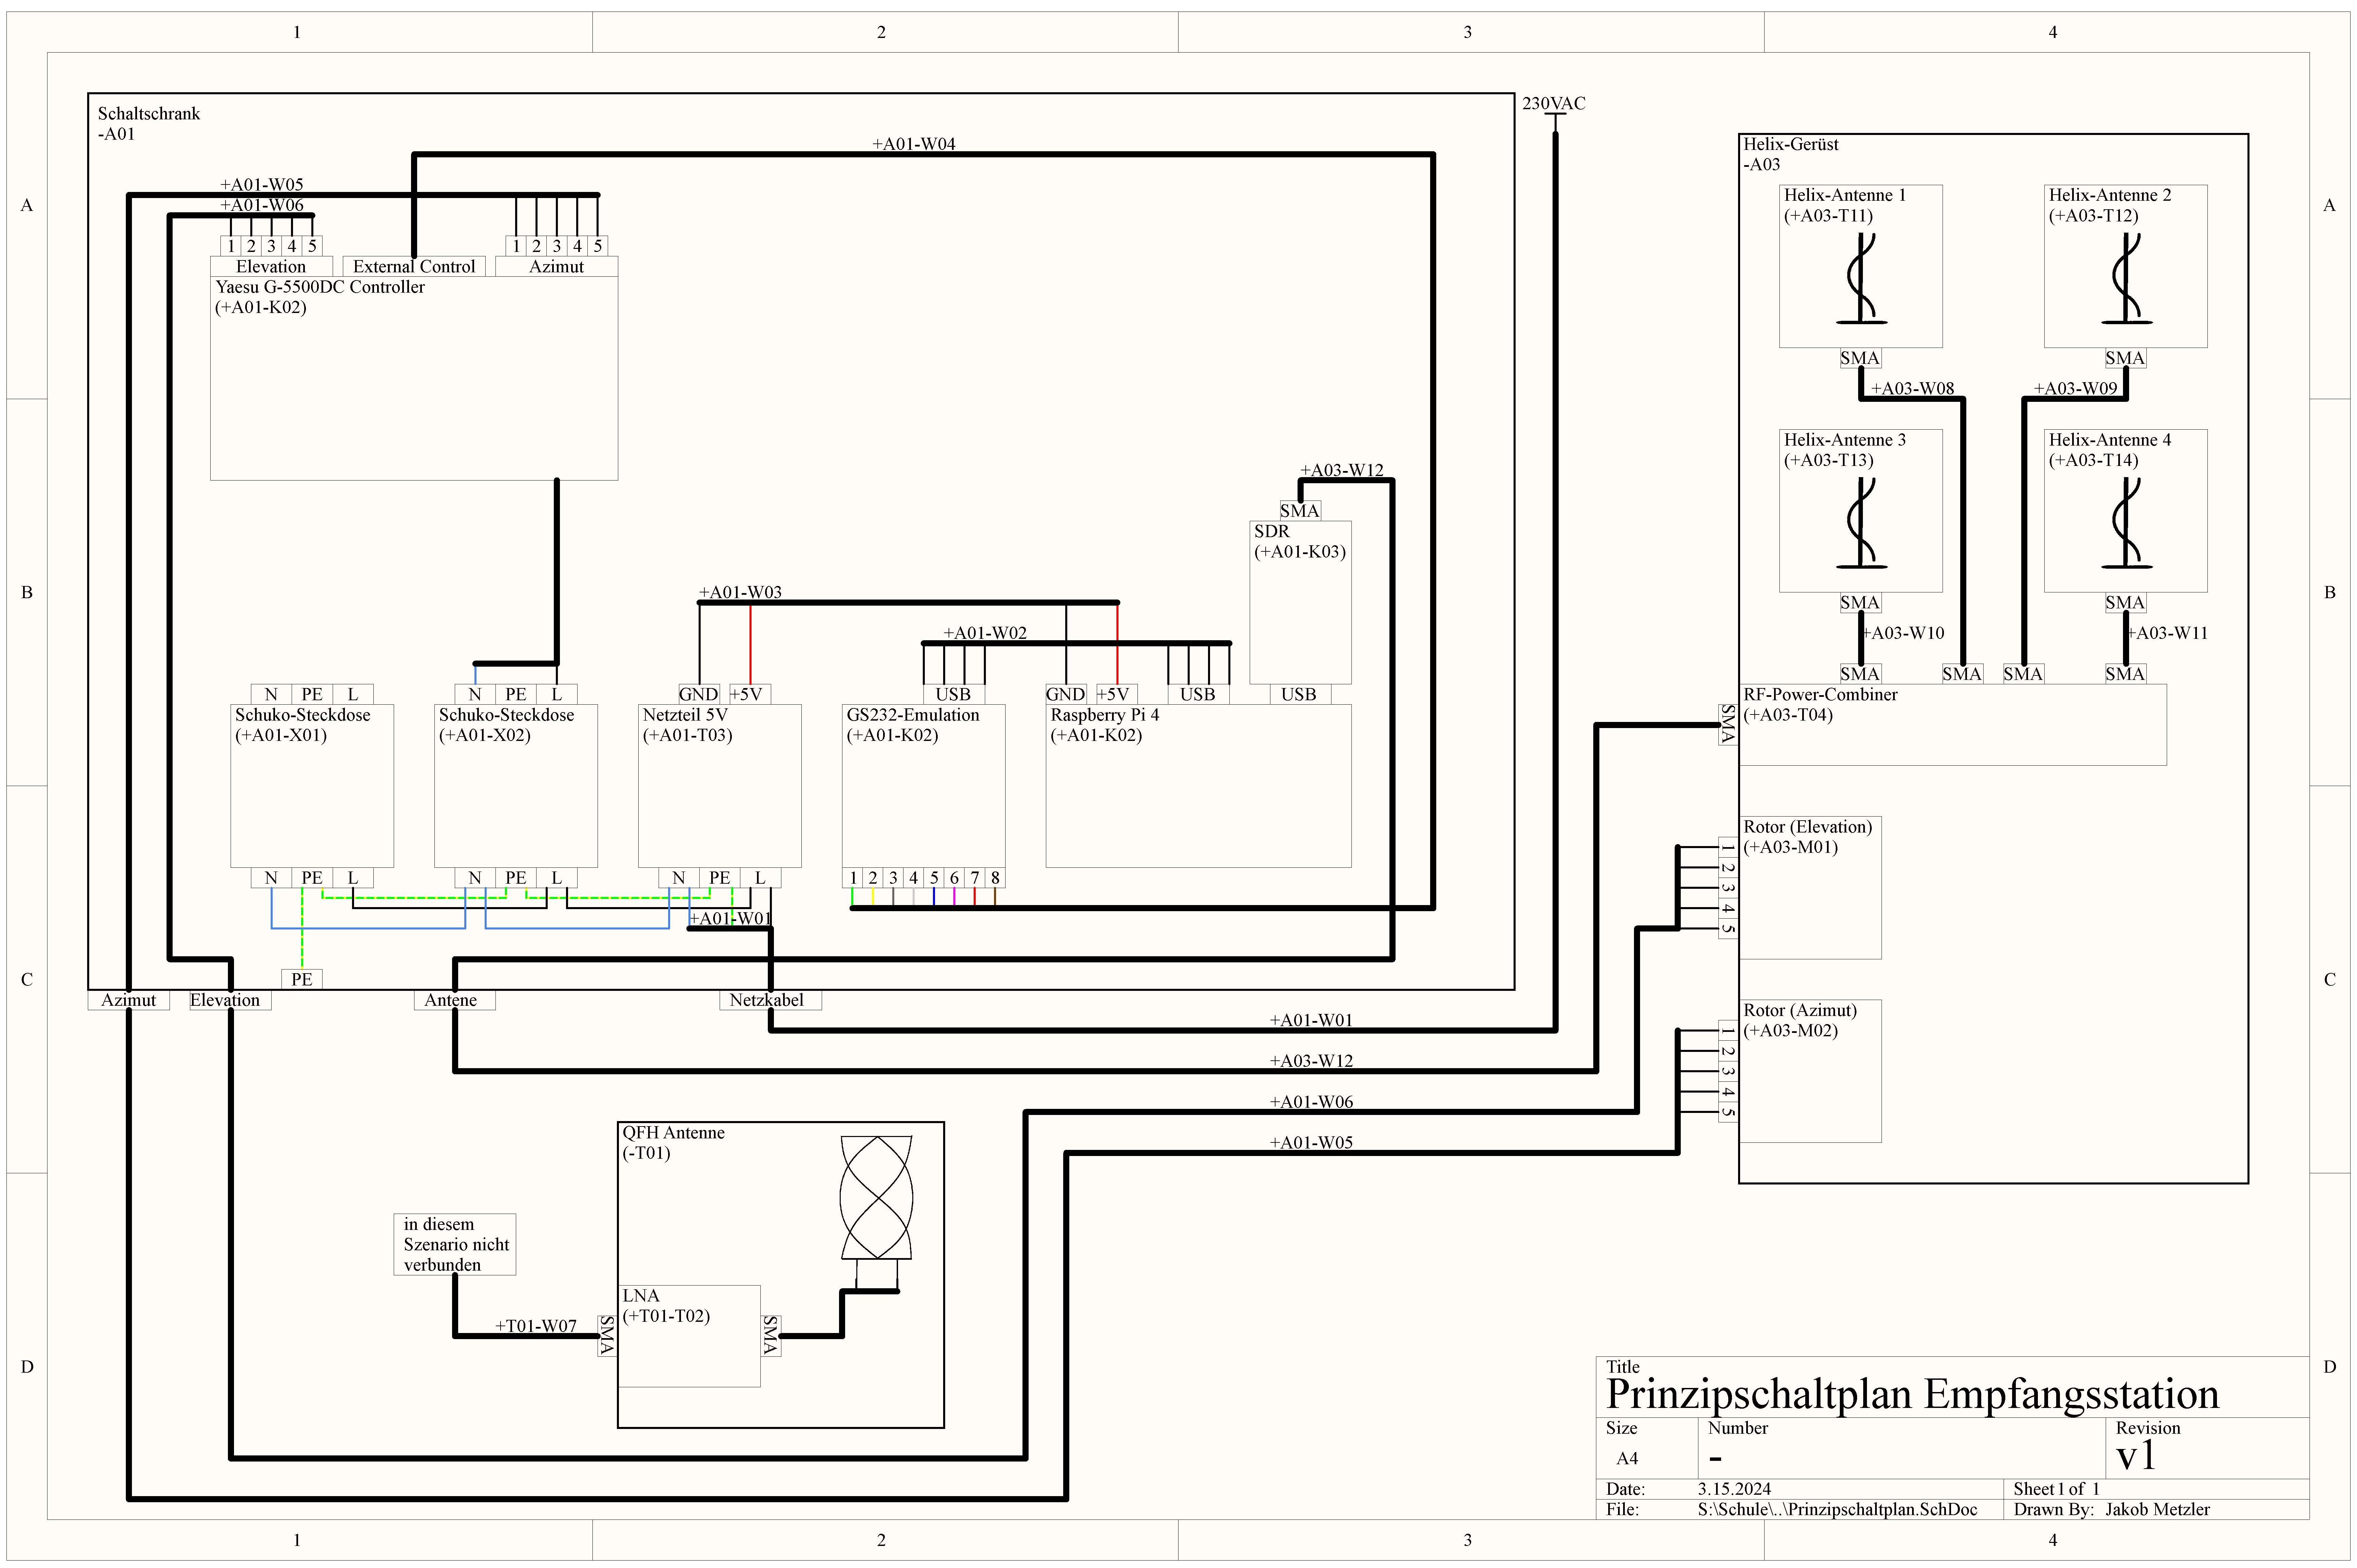
\includegraphics[width=\linewidth]{../ref/Prinzipschaltplan.jpg}
		\caption{Prinzipschaltplan der Empfangsstation}
		\label{fig:prinzipschaltplan}
	\end{figure}
\end{landscape}

\section{Observation planen}
\subsection{Voraussetzung}
Um eine Observation mit der Empfangsstation planen zu können, wird ein Benutzerkonto im SatNOGS Netzwerk mit der entsprechenden Berechtigung benötigt. Folgende Abbildung erläutert die möglichen Aktionen, die gemäß der Art des Benutzerkontos durchgeführt werden können.

\begin{figure} [H]
	\centering
	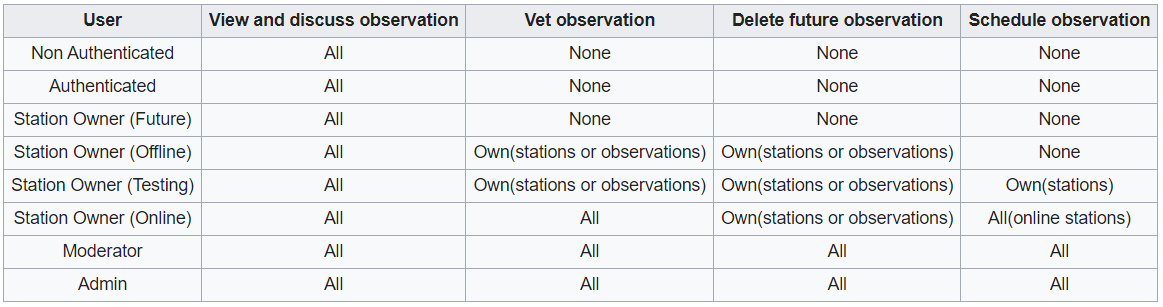
\includegraphics[width=\linewidth]{../ref/network_permission_matrix.png}
	\caption{SatNOGS Netzwerkberechtigungsmatrix \cite{noauthor_operation_nodate}}
	\label{fig:networkpermissionmatrix}
\end{figure}

\subsection{Observation auswählen}
Auf der Seite der Empfangsstation (hier: https://network.satnogs.org/stations/3307/) können über den Reiter \glqq Future Passes\grqq{}  die in der Zukunft passierenden Satelliten angezeigt werden.

\begin{figure} [H]
	\centering
	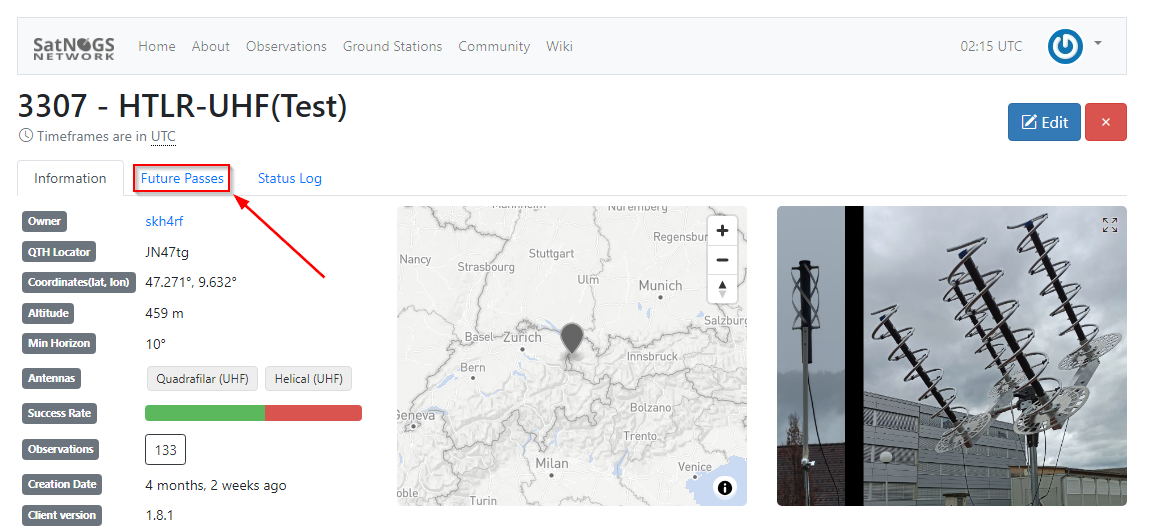
\includegraphics[width=\linewidth]{../ref/schedule_observation_futurepass.png}
	\caption{Landingpage HTLR-UHF(Test) Empfangsstation \cite{noauthor_satnogs_nodate}}
	\label{fig:htrl-uhf(test)landingpage}
\end{figure}

Die folgende Abbildung zeigt die zukünftig passierenden Satelliten und ausgewählte Informationen über die potenzielle Observation.

\begin{figure} [H]
	\centering
	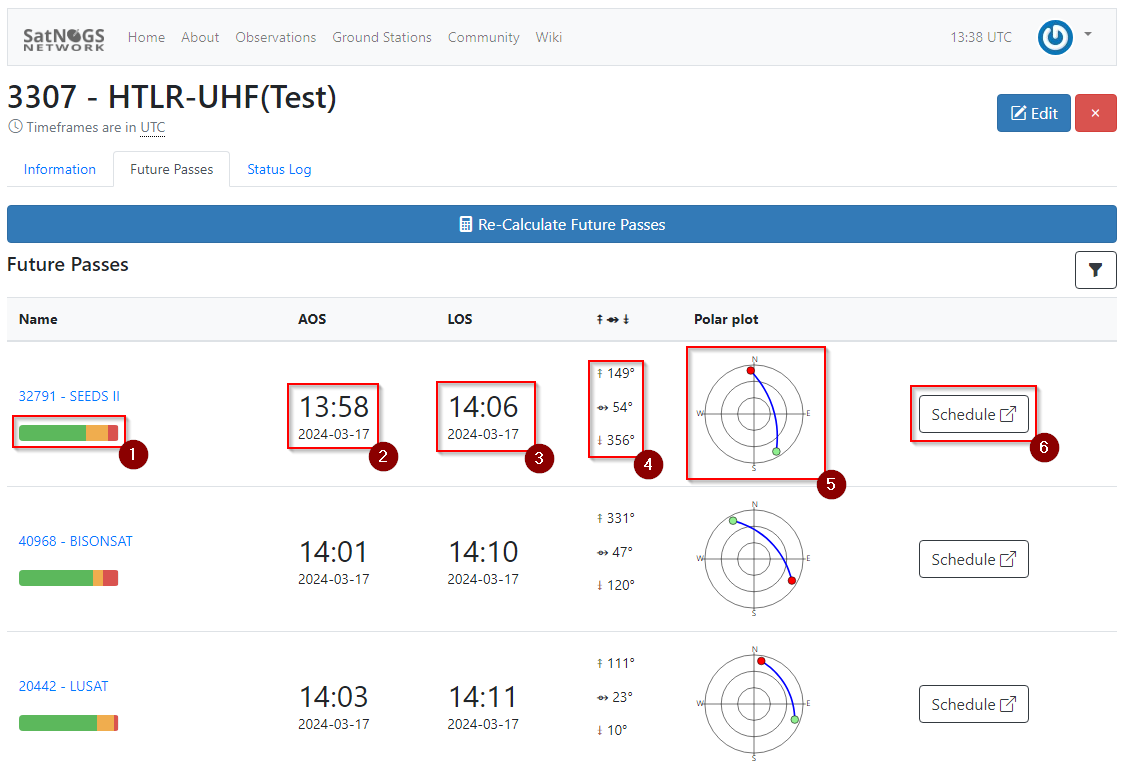
\includegraphics[width=\linewidth]{../ref/schedule_observation_infos.png}
	\caption{HTLR-UHF(Test) Empfangsstation - zukünftige Passierungen \cite{noauthor_satnogs_nodate}}
	\label{fig:htrl-uhf(test)futurepasses}
\end{figure}

Entsprechend der Beschriftung geben die Informationen Aufschluss über folgende Eigenschaften:

\textbf{1}: Status bereits getätigter Observation. Wobei Grün für erfolgreich, Orange für unbewertet, Rot für fehlgeschlagen und Blau für zukünftig steht.\newline

\textbf{2}: Beginn des Signalempfangs (AOS - Acquisition of Signal) \newline

\textbf{3}: Zeitpunkt des Signalverlusts (LOS - Loss of Signal) \newline

\textbf{4}: Von oben nach unten: Azimut zum Zeitpunkt AOS, Azimut zum Zeitpunk der geringsten Entfernung vom Satellit zur Empfangsstation, Azimut zum Zeitpunkt LOS \newline

\textbf{5}: Der Polar-Plot zeigt den Elevationswinkel (Entfernung zum Mittelpunkt) sowie den Azimutalwinkel (Angegeben durch die Himmelsrichtungen) während der Observation an. Der grüne Punkt kennzeichnet den AOS-Zeitpunkt und der rote Punkt den LOS-Zeitpunkt.

Über den mit \textbf{6} markierten Button kann die Observation in einem weiteren Fenster, wie in nachfolgender Grafik gezeigt, konfiguriert und durchgeführt werden.

\begin{figure} [H]
	\centering
	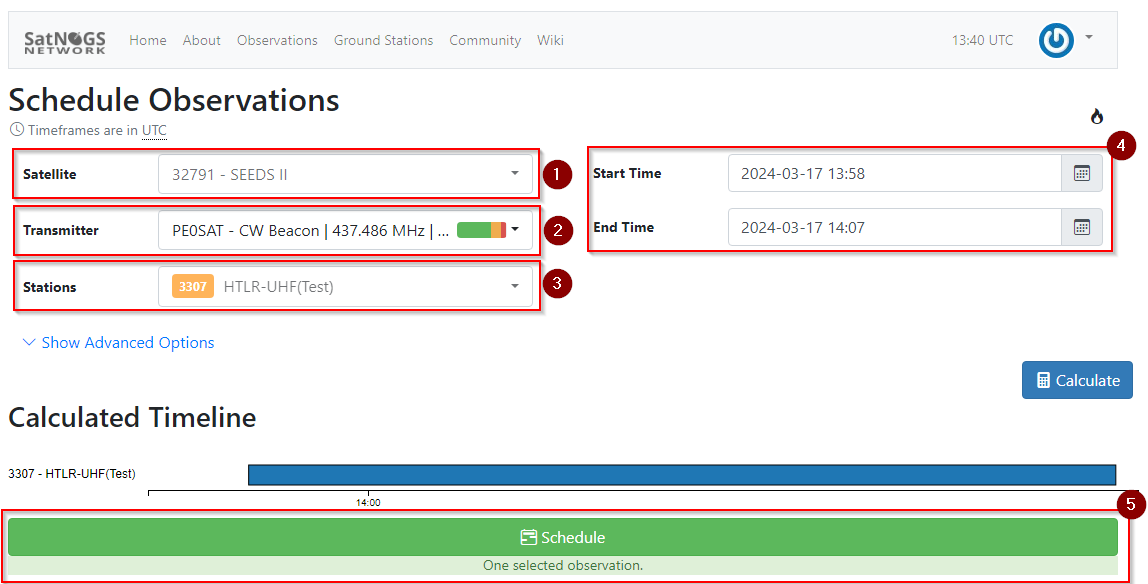
\includegraphics[width=\linewidth]{../ref/schedule_observation_schedule.png}
	\caption{HTLR-UHF(Test) Empfangsstation - Observation konfigurieren und starten} \cite{noauthor_satnogs_nodate}
	\label{fig:htrl-uhf(test)configureobservation}
\end{figure}

Das mit \textbf{1} markierte Dropdown-Menü zeigt den zur Observation ausgewählten Satelliten an und über das mit \textbf{2} Dropdown-Menü markierte können die vorhandenen Sender des Satelliten angezeigt sowie ausgewählt werden. Mithilfe der mit \textbf{4} markierten Eingabefelder kann Start- und Endzeitpunkt der Observation konfiguriert werden. Das mit \textbf{3} markierte Feld zeigt die zur Observation ausgewählte Empfangsstation an. Mit einem Klick auf den mit \textbf{5} markierten Button \glqq Schedule\grqq{} wird die Observation geplant und startet automatisch zum konfigurierten Zeitpunkt.

\subsection{Observation auswerten}
Um die Observationen einer Empfangsstation anzuzeigen, wird auf den in Abbildung \ref{fig:htrl-uhf(test)showobservations} mit \textbf{1} markierten Button auf der Landingpage der Empfangsstation gedrückt.

\begin{figure} [H]
	\centering
	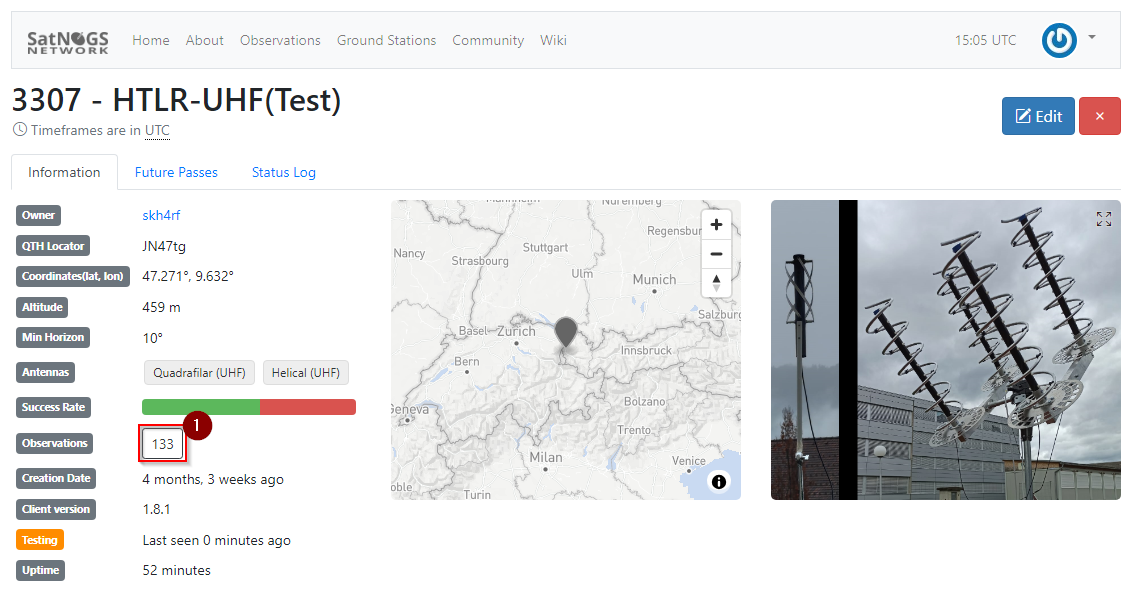
\includegraphics[width=\linewidth]{../ref/show_observation.png}
	\caption{HTLR-UHF(Test) Empfangsstation - Observationen anzeigen} \cite{noauthor_satnogs_nodate}
	\label{fig:htrl-uhf(test)showobservations}
\end{figure}

Die somit erscheinende Übersicht zeigt alle mit dieser Station getätigten und zukünftigen Observationen an.

\begin{figure} [H]
	\centering
	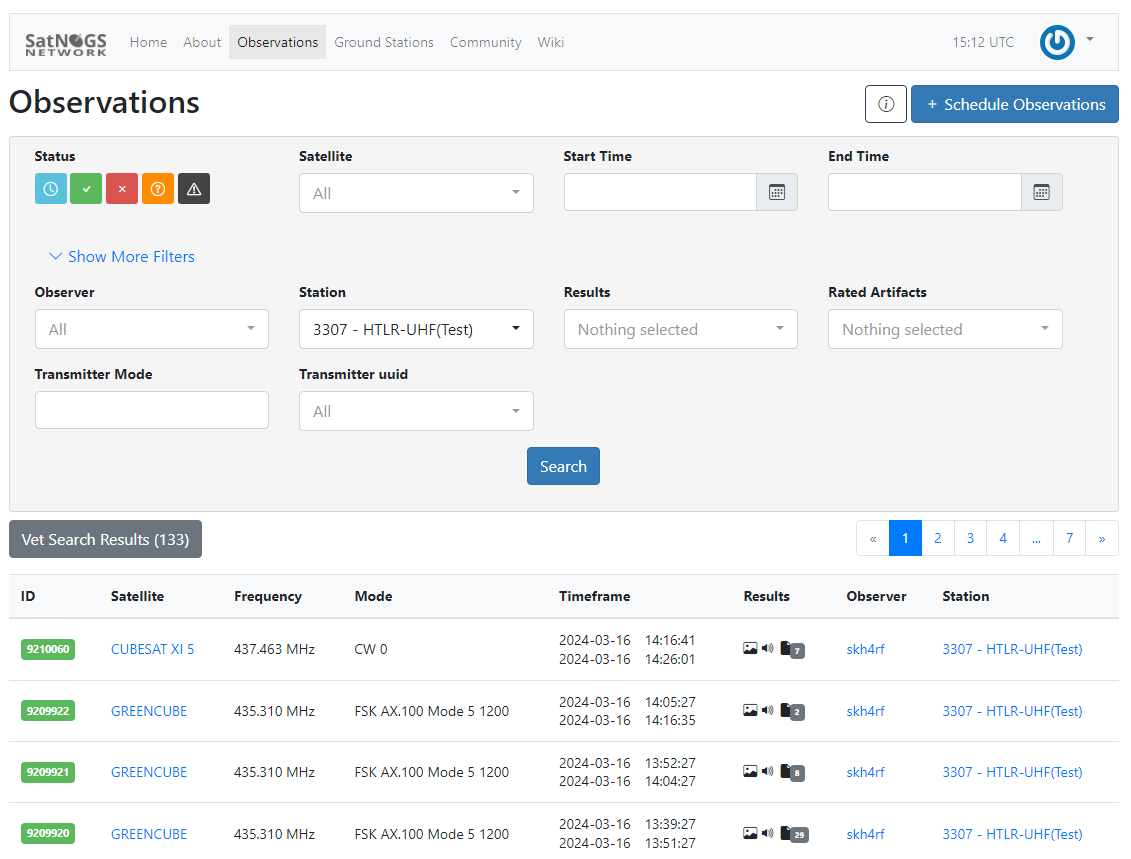
\includegraphics[width=.75\linewidth]{../ref/overview_observations.png}
	\caption{HTLR-UHF(Test) Empfangsstation - Übersicht Observationen} \cite{noauthor_satnogs_nodate}
	\label{fig:htrl-uhf(test)overviewobservations}
\end{figure}

Durch das Klicken auf eine Observation öffnet sich eine weitere Seite, die sowohl die allgemeinen Informationen zur Observation als auch die Ergebnisse in Form eines Wasserfalldiagramms, einer Audiospur sowie von dekodierten Daten enthält. 

\begin{figure} [H]
	\centering
	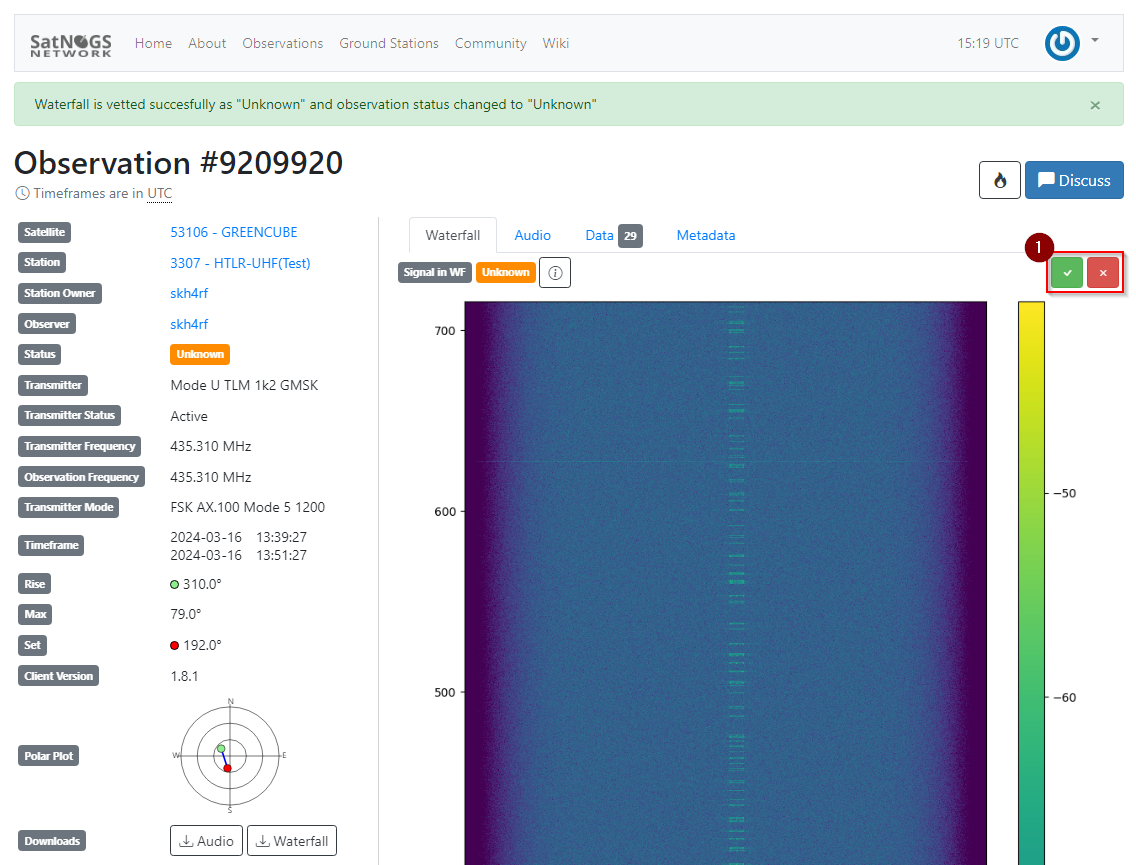
\includegraphics[width=\linewidth]{../ref/vet_observation.png}
	\caption{HTLR-UHF(Test) Empfangsstation - Observation auswerten} \cite{noauthor_satnogs_nodate}
	\label{fig:htrl-uhf(test)vetobservation}
\end{figure}

Ist im Wasserfalldiagramm ein dem Transmitter-Mode entsprechendes Signal zu erkennen, so kann die Observation dementsprechend über die mit \textbf{1} markierten Buttons bewertet werden. Diese Evaluation ist von größer Bedeutung für die Betreiber des Satelliten um dessen Funktionstüchtigkeit zu Überwachen.

\section{SDR-Server starten}
Für die Fehlerbehebung und das Ermitteln der idealen Gain des SDRs ist es vorteilhaft, dieses manuell Bedienen zu können. Eine Möglichkeit hierfür ist das Exportieren der lokal vorhandenen SoapySDR-Geräte, zu welchen auch das RTL-SDR Blog v3 gehört, über das Netzwerk mithilfe eines SoapySDR-Server. Um diesen SoapySDRServer zu starten muss in der SSH des Raspberry Pi 4 lediglich der Befehl \glqq SoapySDRServer --bind="0.0.0.0:55132"\grqq{} ausgeführt werden. \cite{noauthor_soapysdrserver1_nodate}

Wurde der SoapySDRServer auf dem Raspberry Pi 4 gestartet, so kann auf einem weiteren Gerät, welches mit demselben Netzwerk verbunden ist, eine geeignete SDR-Software (zum Beispiel CubicSDR) ausgeführt werden, welches die Steuerung des SDRs ermöglicht.

\begin{figure} [H]
	\centering
	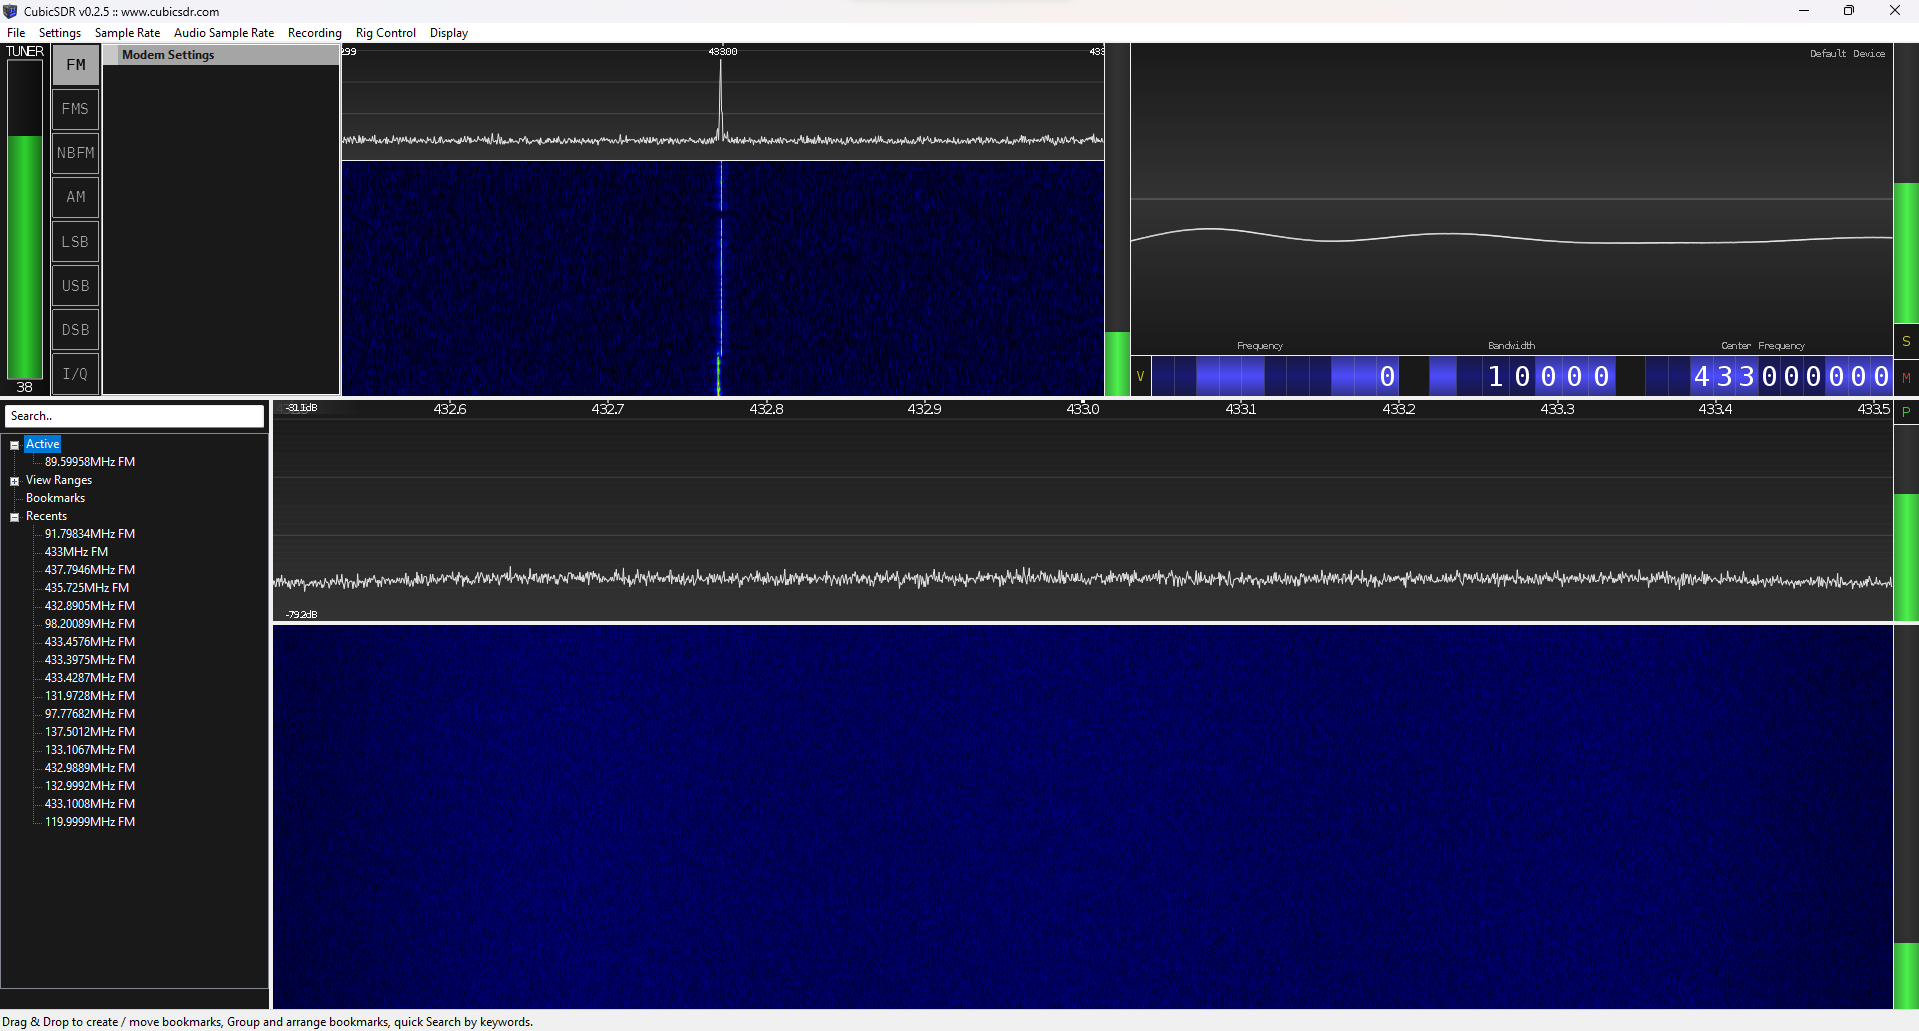
\includegraphics[width=\linewidth]{../ref/OberflaecheCubicSDR.png}
	\caption{Oberfläche von CubicSDR}
	\label{fig:cubicsdr}
\end{figure}


\section{Geeignete Gain ermitteln}
Bei zunehmender Gain-Einstellung eines Empfangssystems wie einem SDR steigt der Rauschpegel, der auch als "Noise Floor" bezeichnet wird, an. Der Noise Floor fungiert als Maß für das Hintergrundrauschen innerhalb des Systems und beschreibt die Gesamtheit aller unerwünschten Signale und Störungen, die vom Empfänger erfasst werden.

Somit wird durch die Erhöhung des Gains nicht nur das Nutzsignal verstärkt, sondern auch das Rauschen. Da das Rauschen unabhängig von der Signalstärke immer vorhanden ist, wird es proportional verstärkt, wenn der Gain erhöht wird. Infolgedessen steigt der Rauschpegel im Verhältnis zum Nutzsignal an, was zu einer Erhöhung des Noise Floors führt. Diese Erhöhung kann die Empfindlichkeit des Empfängers beeinträchtigen und die Fähigkeit, schwache Signale von Hintergrundrauschen zu unterscheiden, einschränken. Folglich ist es von entscheidender Bedeutung, den Gain des Empfangssystems mit Bedacht einzustellen, um eine optimale Signalqualität zu gewährleisten.

Dazu eignet sich die manuelle Steuerung des SDRs über Software-Programme wie CubicSDR. Mithilfe des dort vorhandenen Schiebereglers für die Gain, wird diese solange angehoben bis der Rauschpegel deutlich steigt. In nachfolgender Abbildung ist deutlich zu sehen wie der Rauschpegel ab einer Verstärkung von 30dB signifikant zunimmt. Die Gain des SDRs sollte dementsprechend nicht über 30dB betragen, um auch schwache Signale vom Hintergrundrauschen unterscheiden zu können. 

\begin{figure} [H]
	\centering
	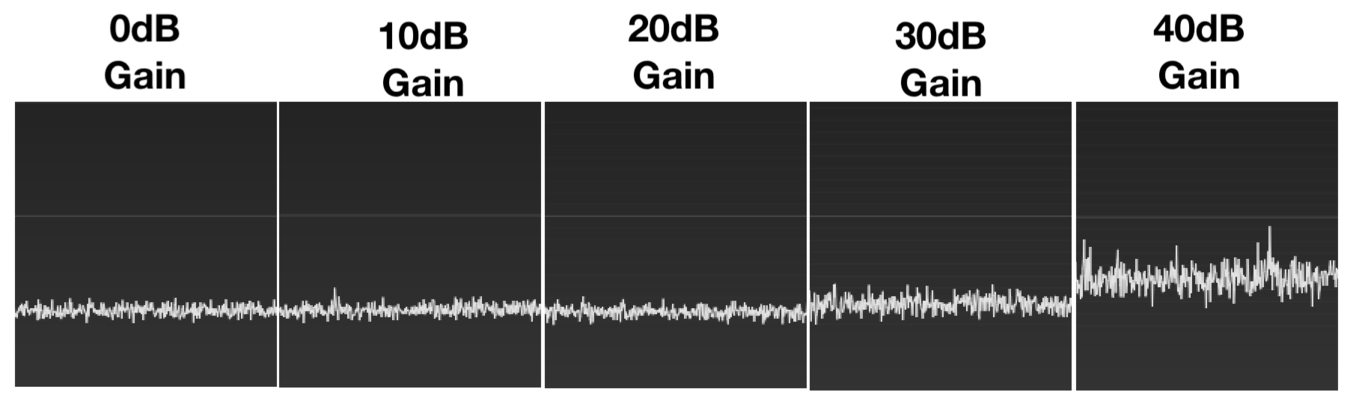
\includegraphics[width=\linewidth]{../ref/noiseflooradjustment.png}
	\caption{Beispielgrafik für den Rauschpegel verschiedener Gains \cite{noauthor_omnidirectional_nodate}}
	\label{fig:noiseflooradjustment}
\end{figure}